\documentclass[a4paper,12pt]{article} % тип документа


\usepackage[T2A]{fontenc} % кодировка
\usepackage[utf8]{inputenc} % кодировка исходного текста
\usepackage[english,russian]{babel} % локализация и переносы

% colors
\usepackage[dvipsnames,table,xcdraw]{xcolor}          
\definecolor{light-blue}{rgb}{0.8,0.85,1}


%symbols
\usepackage{upgreek}
\usepackage{amsmath,amsfonts,amssymb,amsthm,mathtools} %math
% теоремы
\theoremstyle{plain}
\newtheorem{definition}{Определение}[section] 
\newtheorem{theorem}{Теорема}
\newtheorem{example}{Пример}
\numberwithin{equation}{section}



% гиперссылки:
\usepackage{hyperref}
\definecolor{darkblue}{HTML}{0000A0}
\definecolor{linkcolor}{HTML}{0000FF}
\hypersetup{pdfstartview=FitH, citecolor=linkcolor, linkcolor=darkblue,urlcolor=red, colorlinks=true}


% графика:
\usepackage{graphics}
\graphicspath{{pic/}}
\DeclareGraphicsExtensions{.pdf,.png,.jpg, .eps}
\usepackage{caption} % а что без этого летит? (забыл)
\usepackage[section,above,below]{placeins} % управление плавающими объектами (?)
\usepackage{floatflt}
\usepackage{framed}



% работа с таблицами (?)
\usepackage{multirow}
\newcommand{\specialcell}[2][c]{%
	\begin{tabular}[#1]{@{}c@{}}#2\end{tabular}} % перенос строки в ячейке таблицы при пакете multirow


\newcommand{\comment}[1]{} % for multiline comments

% defining red box
\newsavebox{\selvestebox}
\newenvironment{colbox}[1]
{\newcommand\colboxcolor{#1}%
	\begin{lrbox}{\selvestebox}%
		\begin{minipage}{\dimexpr\columnwidth-2\fboxsep\relax}}
		{\end{minipage}\end{lrbox}%
	\begin{center}
		\colorbox[HTML]{\colboxcolor}{\usebox{\selvestebox}}
\end{center}}

% предметный указатель и библиография
\usepackage{makeidx}
\makeindex
\usepackage[nottoc]{tocbibind}

% разметка и стиль (???)
\usepackage[left=2cm, right=2cm, top=2cm, bottom=2cm]{geometry}
\usepackage{fancyhdr}
\pagestyle{fancy}
\fancyhead[L]{\rightmark}
%\lhead{ краткое название}
\chead{}
\rhead{\thepage}
\cfoot{} % get rid of the page number 
\renewcommand{\headrulewidth}{1pt}
\renewcommand{\footrulewidth}{0pt}
\usepackage{indentfirst}

\usepackage{framed}
\usepackage{fancyvrb} %for fraim aroun verbatim
 % основная шапка

\usepackage{graphicx} 

\author{Юрий Голубев\\ yura.winter@gmail.com }
\title{Задачи по теории вероятностей}
\date{\today}

\usepackage{bbm} % for \mathbbm

\usepackage{float} % for fix table

\begin{document}
\maketitle

\begin{abstract}
Задачи по теории вероятностей
\end{abstract}
%%%%%%%%%%%%%%%%%%%%%%%%%%%%%%%%%%%%%%%%%%%%%%%%%%%%%%%%%%%%%%	
\tableofcontents

\section*{Предисловие}
\addcontentsline{toc}{section}{Предисловие}

Задачи по теории вероятностей.





\clearpage
\part{Первое задание}


\section{Задачи на теорию множеств}

\begin{example}\textbf{T 1}


Пусть $A, B-$ два события. Найти все события $X$ такие, что 
$\overline{(X \cup A)} \cup \overline{(X \cup \bar{A})}=B$

По правилу де Моргана: 
$$
\overline{B}=
(X \cup A) \cap (X \cup \bar{A})
$$

По правилу де Моргана $(X \cup \bar{A})= (\overline{\overline{X} \cap A})$, таким образом:
$$
(X \cup A) \cap (\overline{\overline{X} \cap A}) =
\overline{\overline{(X \cup A)} \cup (\overline{X} \cap A) }=
\overline{(\overline{X} \cap \overline{A}) \cup (\overline{X} \cap A)}= X
$$


Ответ $ X=\overline{B}$.

\end{example}


\begin{example}\textbf{T2}

Пусть $A, B-$ два события. Найти все события $X$ такие, что $A X=A B \Longleftrightarrow  A \cup X=A \cup B$.

Очевидно, что необходимо, чтобы $X\in A\cap B$. Но также $X$ может содержать любое множество $ Y\in X $, которое при $A \cup X$ дало бы ноль, таким образом задача решена.

Ответ $ X=Y \cup (A\cap B)  \ \forall \ Y\in \overline{A}$.


\end{example}


\begin{example}\textbf{T3}

Пусть $A_{1}, \ldots, A_{n}-$ события. Покажите, что
$$
\mathrm{P}\left(\bigcup_{k=1}^{n} A_{k}\right)+\mathrm{P}\left(\bigcap_{k=1}^{n} \overline{A_{k}}\right)=1
$$

Воспользуемся свойству вероятностной меры: $\forall B \quad \mathrm{P}(B)+\mathrm{P}(\overline{B})=1$. 
Возьмем в качестве $B$ выражение: $B=\bigcup_{k=1}^n A_k$, тогда 
$\overline{B}=\bigcap_{k=1}^n\overline{A}$.
Подставляя, получаем:
$$
\mathrm{P}\left(\bigcup_{k=1}^{n} A_{k}\right)+\mathrm{P}\left(\bigcap_{k=1}^{n} \overline{A_{k}}\right)=1
$$


\end{example}




\begin{example}\textbf{T4}

Пусть $A_{1}, A_{2}, \ldots$ - последовательность событий и $\mathrm{P}\left(A_{n}\right)=1$ для всех $n=1,2, \ldots .$ Покажите, что
$$
\mathrm{P}\left(\bigcap_{n=1}^{\infty} A_{n}\right)=1
$$


Первый способ:
Пусть $B_n= \bigcap_{i=1}^{n} A_{i} $. Заметим, что $ B_1\in B_2 \in \ldots$, тогда 
\[ P(\overline{B_n})=P(bigcap_{i=1}^{n}\overline{ A_{i}}) \le \sum_{i=1}^{n} P(\overline{A_i})=0 \]

Поэтому в силу положительной определенности $ P(\overline{B_n})=0,$ поэтому $ P(B_n)=1 $

Окончательно, заменяя $A$ на $B$ и используя непрерывность вероятностной меры получаем:
$$
\mathrm{P}\left(\bigcap_{n=1}^{\infty} A_{n}\right)=
\mathrm{P}\left(\lim\limits_{n\rightarrow\infty} B_{n}\right)=
\lim\limits_{n\rightarrow\infty} \mathrm{P} (B_{n})
$$






Второй способ: знаем, что на всем вероятностном пространстве $\Omega$ выполняется $\mathrm{P}(\Omega)=1.$ 
Таким образом $A_i=\Omega-A_{i0}$, где $ A_{i0}: \mathrm{P}(A_{i0})=0$.
Таким образом, 
$$
\mathrm{P}\left(\bigcap_{n=1}^{\infty} A_{n}\right)=
\mathrm{P}\left(\Omega-\bigcap_{n=1}^{\infty} A_{i0}\right)=
1-\sum_{n=1}^{\infty} 0=1
$$








\end{example}


\begin{example}\textbf{T5}

Пусть $A_{1}, A_{2}, \ldots$ - последовательность событий. Покажите, что
$$
P\left(\varliminf_{n \rightarrow \infty} A_{n}\right) \leq 
\varliminf_{n \rightarrow \infty} \mathrm{P}\left(A_{n}\right) \leq 
\varlimsup_{n \rightarrow \infty} \mathrm{P}\left(A_{n}\right) \leq 
\mathrm{P}\left(\varlimsup_{n \rightarrow \infty} A_{n}\right)
$$

Вспомним определение:
\[ 
A^{*}=\varlimsup_{n \rightarrow \infty} A_{n}=
\bigcap_{n=1}^{\infty} \bigcup_{k \geqslant n} A_{k}, \quad 
A_{*}=\varliminf_{n \rightarrow \infty} A_{n}=\bigcup_{n=1}^{\infty} \bigcap_{k \geqslant n} A_{k} 
\]


Первое неравенство доказывается с помощью непрерывности вероятностной меры:
\[ P\left(\varliminf_{n \rightarrow \infty} A_{n}\right) =
P(\bigcup_{n=1}^{\infty} \bigcap_{k \geqslant n} A_{k})\equiv
P(\bigcup_{n=1}^{\infty} B_n) \equiv
P(\lim B_n)
\underbrace{=}_{ \text{по непрер. меры} }^{\text{т.к.} B_1\subset B_2 \subset\ldots}
\lim P(B_n)\underbrace{\le}_{ B_n=\cup_{N=n}^{\infty}\subset A_n } \varliminf_{n \rightarrow \infty} P(A_n)
\]





Выражение 
$ \varliminf_{n \rightarrow \infty} \mathrm{P}\left(A_{n}\right) \leq 
\varlimsup_{n \rightarrow \infty} \mathrm{P}\left(A_{n}\right)
$ 
очевидно.


И последнее неравенство:
\[ P(\varlimsup_{n \rightarrow \infty} A_n)=
P(\bigcup_{n=1}^{\infty} \bigcap_{k \geqslant n} A_{k})\equiv
P(\bigcup_{n=1}^{\infty} B_n) \equiv
P(\lim B_n)
\underbrace{=}_{ \text{по непрер. меры} }^{\text{т.к.} B_1\supset B_2\supset\ldots}
\lim P(B_n)\underbrace{\ge}_{ B_n=\cup_{N=n}^{\infty}\supset A_n } P(A_n) \]






\end{example}




\begin{example}\textbf{T6}

Покажите, что для любых двух событий $A$ и $B$ выполняется неравенство
$$
|\mathrm{P}(A B)-\mathrm{P}(A) \mathrm{P}(B)| \leq \frac{1}{4}
$$

Обозначим $ A B\equiv c$, $ A\backslash B\equiv a$, $ B\backslash A\equiv b$, тогда доказать нужно нам, что
$$ |c-(a+c)(b+c)|\le \frac{1}{4} $$

Причем по условию, так как мы работаем с событиями, должно выполняться: $ a+b+c\le 1$.

Докажем, что $ c-(a+c)(b+c)\ge -\frac{1}{4}$. Действительно, $ 2\sqrt{ab}\le a+b\le 1 \rightarrow ab\le 1\frac{1}{4}$.
\[ c-(a+c)(b+c)=с(1-\underbrace{-a-b-c}_{\le 0})-ab \ge -\frac{1}{4}\]



Докажем, что $ c-(a+c)(b+c)\le \frac{1}{4}$. Преобразуем выражение уже в другом виде:
\[ c-(a+c)(b+c)\le c-c^2=c(1-c)=(\sqrt{c}\sqrt{(1-c)})^2\underbrace{\le}_{\text{неравнство Коши}}
\left(\frac{1}{2} ( c + ( 1-c ))
\right)^2 \le\frac{1}{4}\]

Таким образом, уж точно
$$ |c-(a+c)(b+c)|\le \frac{1}{4}. $$

\end{example}






\section{Простые жизненные задачи}


\begin{example}\textbf{T7}

Что вероятнее, получить хотя бы одну единицу при бросании четырех игральных костей 
или хотя бы одну пару единиц за один бросок при 24 бросаниях двух костей?

Посмотрим на случай четырех костей.

Можно считать количество успешных исходов, но это сделать сложно, так что пойдем от обратного, посчитаем неудачные исходы.

Вероятность невыпадения единицы в одном испытании: $ 1-\frac{1}{6}=\frac{5}{6}$, в четырех экспериментах вероятность того, что среди всех выпавших костей нет ни одной единицы равна $ \left(\frac{5}{6} \right))^4$. 

Тогда вероятность выпадения единицы равна 
$$P_1= 1- (\frac{5}{6})^4$$


Посмотрим на случай двух костей.
При одном бросании двух костей у нас 36 может быть разных исходов, при этом подходит только один.
Поэтому  аналогично первому пункту, вероятность хотя бы за какой-то бросок получить пару единиц, равна:
$$P_2= 1-(1-\frac{1}{36})^{24}=1-\left(\frac{35}{36} \right)^{24} $$

Осталось только сравнить эти $ P_2$ и $ P_1$. Просто посчитаем их на калькуляторе. В итоге 
\[ P_1> P_2 \]


Ответ: Успех в случае бросания одной кости имеет большую вероятность.


\end{example}



\begin{example}\textbf{T8}

Объяснить, почему при подбрасывании трёх игральных костей 11 очков выпадают чаще, чем 12.


Посчитаем количество исходов, которые дадут 11 очков в сумме. По сути это количество целочисленных положительных решений уравнения $ x_1+x_2+x_3=11$ при условии $ x_1,x_2,x_3\le 6$.
%
%
\[ P(x_1+x_2+x_3=11)=\sum_{i=1}^{6} P(a=i) P(x_2+x_2=11-i)=\frac{1}{6}\sum_{i=5}^{10} P(x_2+x_2=i) \]
%
\[ P(x_1+x_2+x_3=12)=\sum_{i=1}^{6} P(a=i) P(x_2+x_2=12-i)=\frac{1}{6}\sum_{i=6}^{11} P(x_2+x_2=i) 
\]
%
\[P(x_1+x_2+x_3=12)-P(x_1+x_2+x_3=12)=P(x_2+x_3=11)-P(x_2+x_3=5)
\underbrace{=}_{\text{ исходы}}^{\text{считаем благоприятные} } \frac{2}{36}-\frac{4}{36}<0  \]

Поэтому при подбрасывании трёх игральных костей 11 очков выпадают чаще, чем 12.



\end{example}




\begin{example}\textbf{T9}. 

Из колоды в 52 карты наудачу берется 6 карт. 
Какова вероятность того, что среди них будут представительницы всех четырех мастей?

Назовем наши масти А, В, С, D. Назовем $ A_A, A_B, A_C, A_D$ - исходы, в которых есть масть А, В, С, D соответственно.

Нам нужно событие $ X= A_A \cap A_B \cap A_C \cap A_D$ - что есть представители всех мастей.

Посчитаем вероятность события $ \overline{X}= \overline{A_A} \cup \overline{A_B} \cup \overline{A_C} \cup \overline{A_D}$ -
что нет представителя какой-то из мастей.
Для этого воспользуемся формулой включения-исключения:
\[ \mathbf{P}\left\{\bigcup_{k=1}^{n} A_{k}\right\}=
\sum_{m=1}^{n}(-1)^{m-1} 
\sum_{1 \leqslant i_{1}<\ldots<i_{m} \leqslant n} 
\mathbf{P}\left\{A_{i_{1}} A_{i_{2}} \ldots A_{i_{m}}\right\} 
\]
И так как одной из четырех масти не может быть - 4мя способами, двух мастей - $C_4^2=6$ способами, трех - $C_4^3=4$ способами, то вторая сумма, 
учитывая что вероятности наличия разных мастей не зависят от конкретного вида масти, будет иметь вид:
\[ \mathbf{P}\left\{\bigcup_{k=1}^{n} A_{k}\right\}=
4 \mathbf{P}(\overline{A_1})-
6 \mathbf{P}(\overline{A_1}\overline{A_2})
+3 \mathbf{P}(\overline{A_1}\overline{A_2} \overline{A_3} )  \]

Посчитаем вероятности членов в этой сумме, найдя количество благоприятствующих исходов:
\[ P(\overline{A_i})=\frac{C_{52-13}^6}{C_{52}^6}; 
\quad 
P(\overline{A_i})=\frac{C_{52-13-13}^6}{C_{52}^6}; 
P(\overline{A_i})=\frac{C_{52-13-13-13}^6}{C_{52}^6}; 
\]


Подставим все в ответ: $ P_{\text{искомое}}=
1-\left( 4 \frac{C_{39}^6}{C_{52}^6} -6 \frac{C_{26}^6}{C_{52}^6} + 4 \frac{C_{13}^6}{C_{52}^6}\right) $









\end{example}


\begin{example}\textbf{T 10}

В $n$ конвертов разложено по одному письму $n$ адресатам. 
На каждом конверте наудачу написан один из $n$ адресов. 
Найти вероятность того, что хотя бы одно письмо пойдет по назначению.

Пусть $ A_i$ - элементарное событие, состоящее в том, что $i$-е письмо дошло своему адресату. Тогда нужно найти.
\[ \mathbf{P}(\bigcup_{i=1}^n A_i)= \sum_{m=1}^{n}(-1)^{m-1} \sum_{1 \leqslant i_{1}<\cdots<i_{m} \leqslant n}
\mathbf{P}\left(A_{i_{1}} A_{i_{2}} \cdots A_{i_{m}}\right) \]

Посмотрим на каждое слагаемое внимательнее. Каждое слагаемое - вероятность того, что у нас будет $m$ попаданий конвертов и писем.
Если зафиксировать $m$ писем, то оставшиеся письма можно раскладывать $(n-m)!$ способами. 
Всего можно $n$ писем по $n$ конвертам разложить $ n!$ способами:
\[ \mathbf{P}\left(A_{i_{1}} A_{i_{2}}\cdots A_{i_{m}}\right)=\frac{(n-m)!}{n!} \]
при этом при любых перестановках адресатов вероятность такая же, а всего перестановок при фиксированном $m$ будет $ C_n^m$.
В итоге формула примет вид:
\[ \mathbf{P}=\sum_{m=1}^{n}(-1)^{m-1} C_n^m \frac{(n-m)!}{n!}=
\sum_{m=1}^{n}(-1)^{m-1}\frac{1}{m!} \]

Ответ: $\mathbf{P}= \sum_{m=1}^{n}(-1)^{m-1}\frac{1}{m!} $

\end{example}






\begin{example}\textbf{T11}

У билетной кассы стоит очередь в 100 человек. Половина людей в очереди имеет 100-рублевые купюры, а вторая половина - 50-рублевые купюры. 
Изначально в кассе нет денег и стоимость билета - 50 рублей. 
Какова вероятность, что никому не придется ждать сдачу?

Для каждого человека, имеющего 100р чтобы нашлась сдача необходимо, чтобы был перед ним человек, пришедший с 50р.


Таким образом, задача эквивалентна задаче о скобочной последовательности, где есть открывающая и закрывающая скобка. и каждая открытая должна иметь после нее закрывающую.


Известно, что число скобочных последовательностей из $ n$ открывающих и $ n$ закрывающих скобок равно числу Каталана $K_n = \frac{1}{n+1}C_n^{2n}$.

Всего же возможных последовательностей - число сочетаний $ C_{2n}^n$, Поэтому ответ: $P= \frac{1}{n+1}$, для нашего случая, $ n=50$, имеем $P= \frac{1}{51}$


Ответ: $P= \frac{1}{51}$


\end{example}


\begin{example}\textbf{T12}

Расстояние от пункта А до пункта В автобус проходит за 2 минуты, а пешеход - за 15 минут. 
Интервал движения автобусов 25 минут. 
Пешеход в случайный момент времени из пункта А и отправляется в В пешком. 
Найти вероятность того, что в пути пешехода догонит очередной автобус.

Будем решать графически.
Нарисуем 2D пространство-время, как на картинке.


\begin{figure}[h!]
\centering
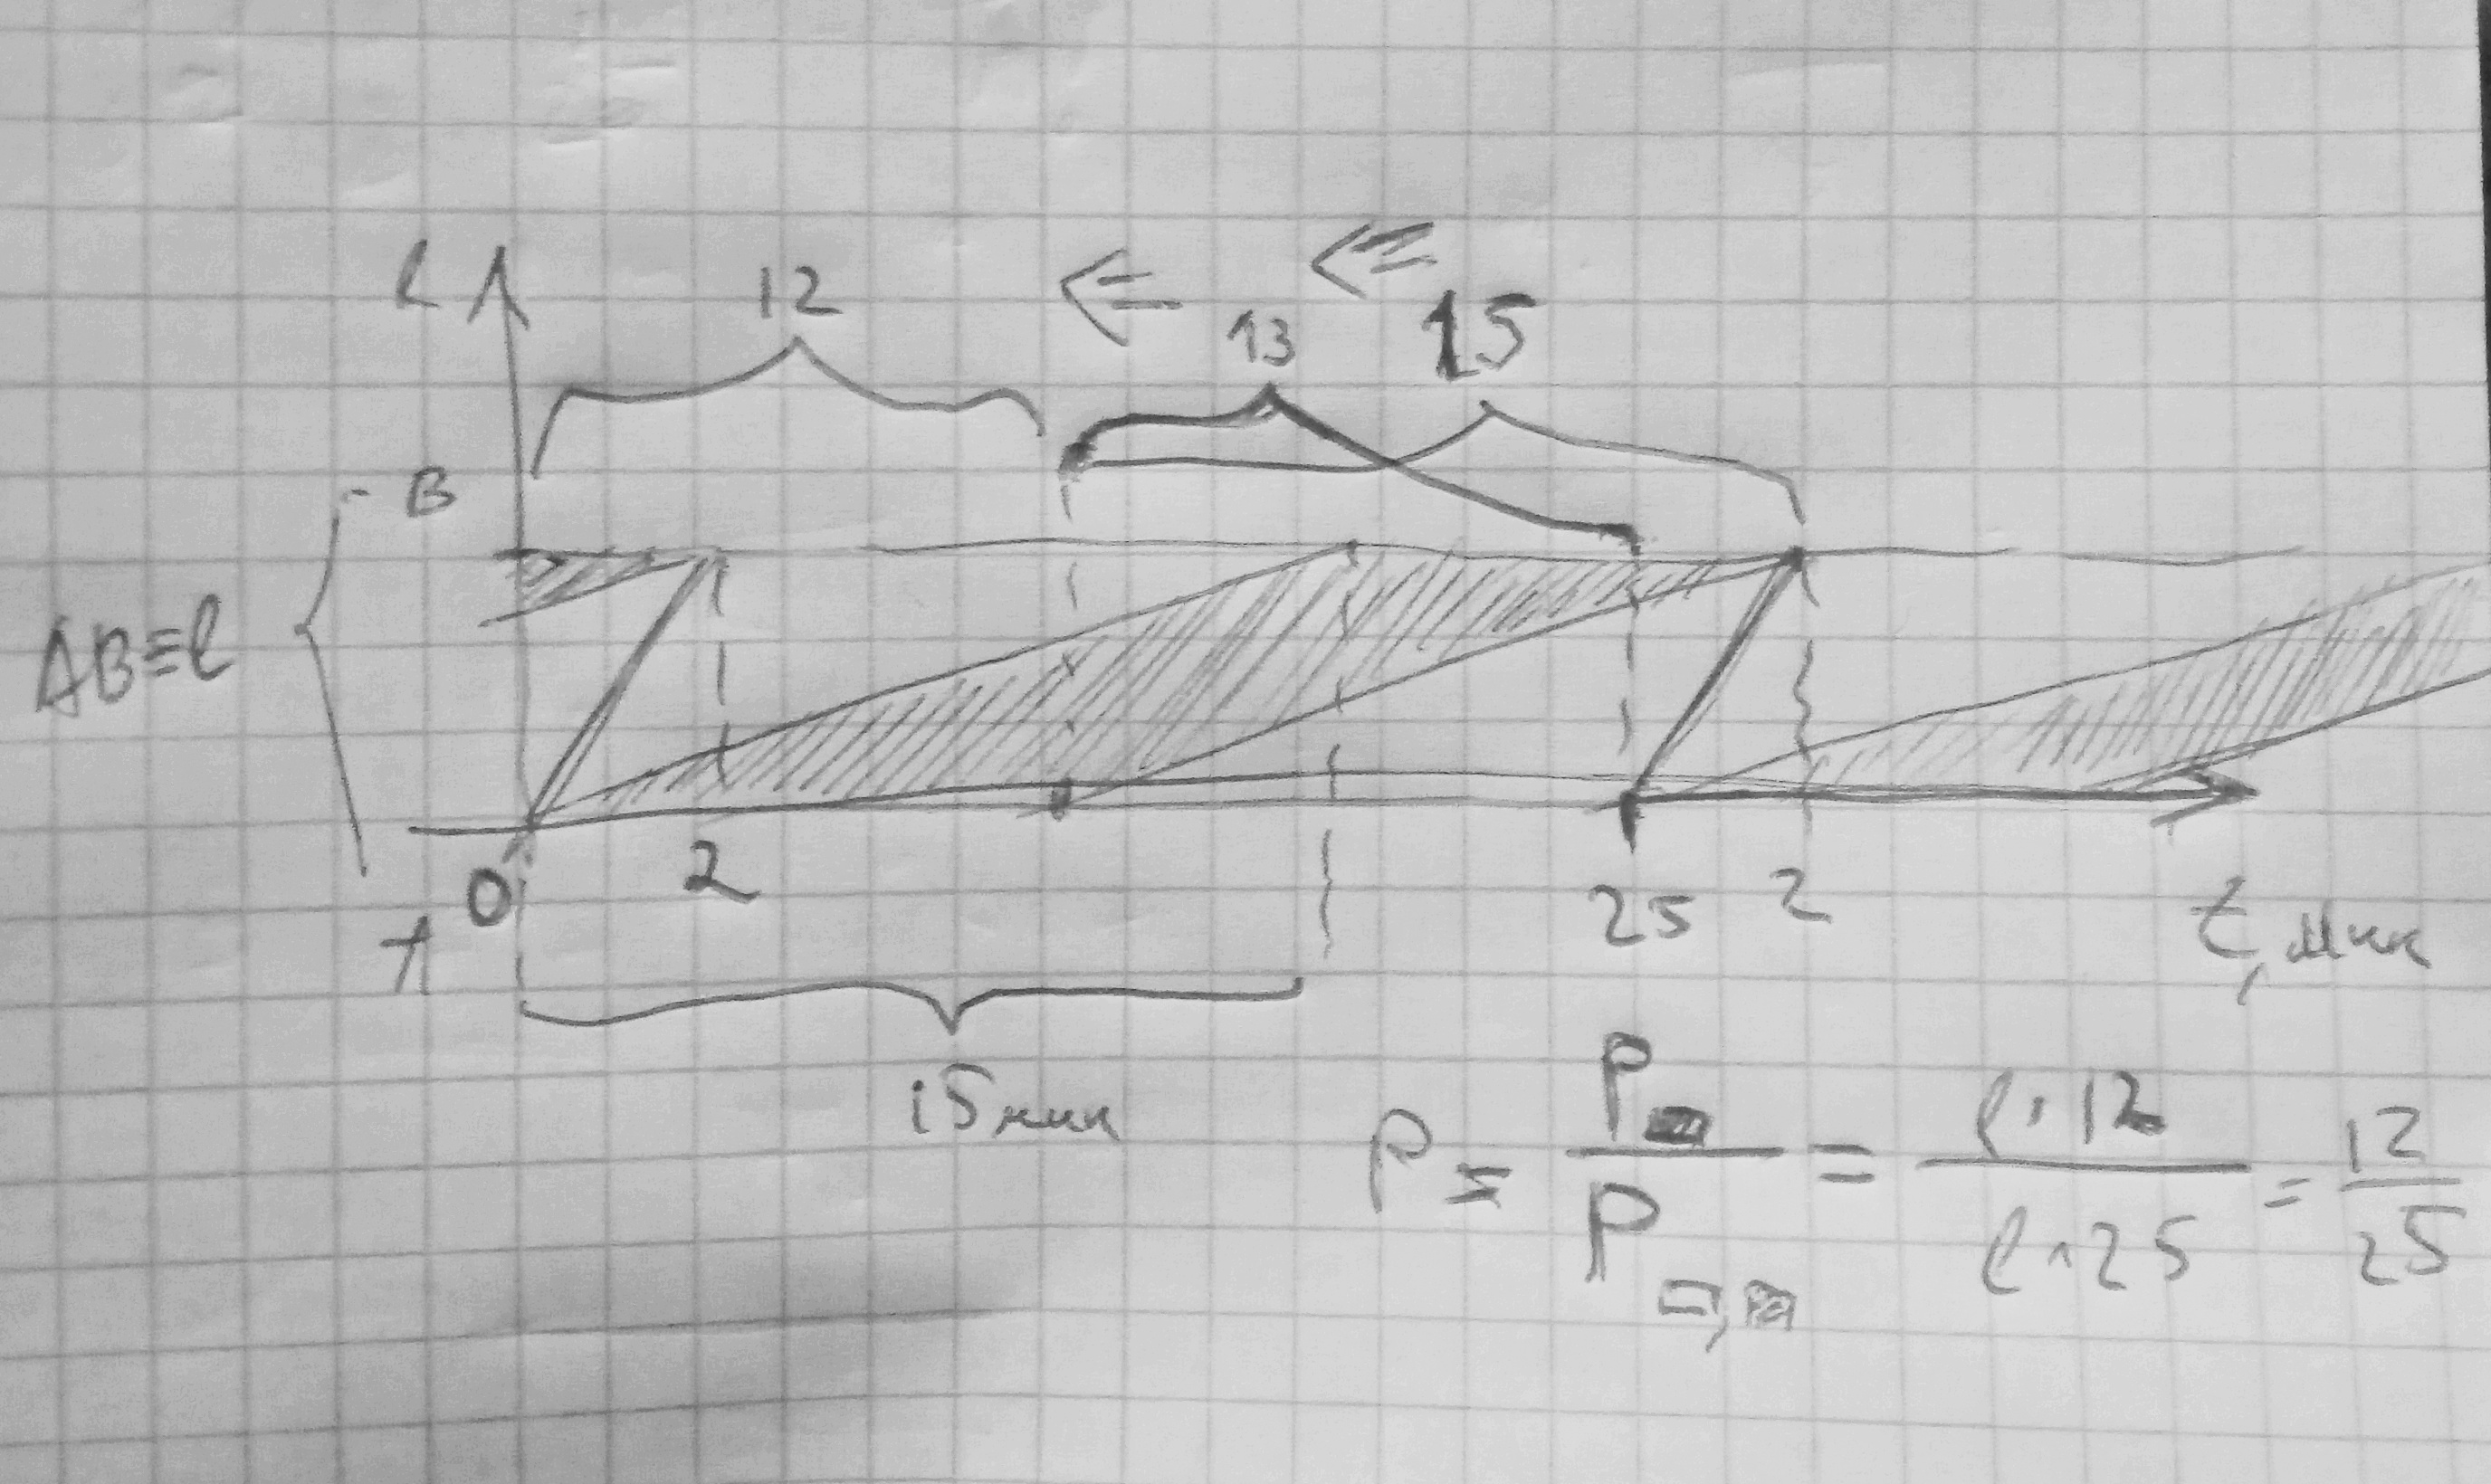
\includegraphics[width=0.5\linewidth]{t12}
\caption{для задачи Т12. 
Здесь короткая линия под наклоном - линия движения автобусе. длинные наклонные линии - линии движения человека. заштрихованная область - область всех возможных линий, где мировая линия человека не пересечет мировую линию автобуса. 
(я рисовал рисунок, решая обратную задачу, поэтому там написано $\frac{12}{25}$)}
\label{fig:t12}
\end{figure}

Несложные соображения показывают, что незаштрихованная область, которая соответствует встрече, может быть такой такой.


Таким образом, вероятность не встречи равна отношению площади этой области к интервалу, в котором мы смотрим движение автобуса. То есть вероятность равна: $\frac{15-2}{25}=\frac{13}{25} $

Ответ: $\frac{13}{25} $

\end{example}


\begin{example}\textbf{T13}


\begin{figure}[h!]
\centering
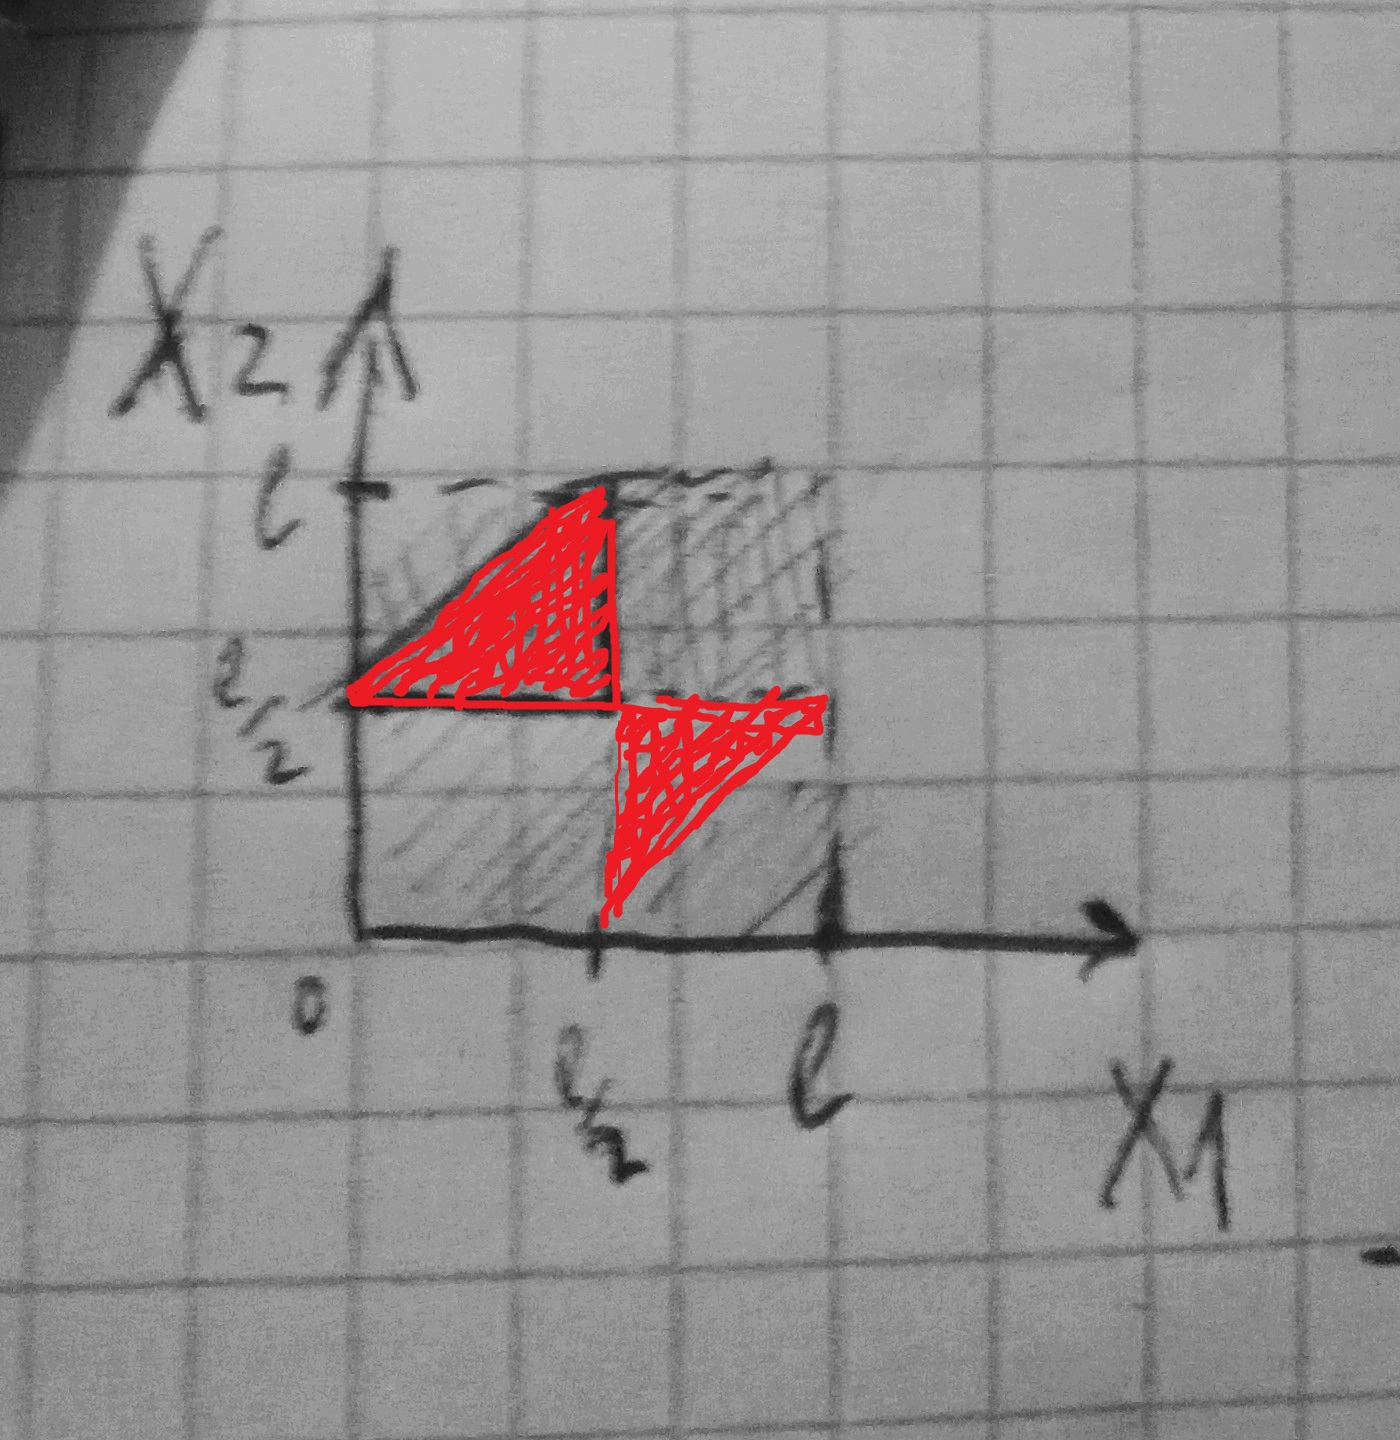
\includegraphics[width=0.2\linewidth]{t13}
\caption{геометрическая вероятность для задачи Т13}
\label{fig:t13}
\end{figure}

На отрезке наудачу выбираются две точки. 
Какова вероятность того, что из получившихся трех отрезков можно составить треугольник?

Треугольник можно составить если для любых сторон его $ a,b,c$ выполняется $ a<c+b$. 
То есть $ 2c<+b+c=l$, поэтому любая сторона его должна быть меньше $\frac{l}{2}$.
Введем координаты $ a=\min (x_1, x_2), b=|x_2-x_1|, c=l -\max (x_1, x_2)$

У нас должно выполняться при $ x_1<x_2 $:
\[ x_1<\frac{l}{2}; x_2>\frac{l}{2}; x_2-x_1> \frac{l}{2} \]

А при $ x_1>x_2 $:
\[ x_1>\frac{l}{2}; x_2<\frac{l}{2}; x_2-x_1< \frac{l}{2} \]



Изобразим это на рисунке, посчитаем долю площади от всего квадрата, запишем ответ.


В итоге нужная нам область составляет $ \frac{1}{4}$ от площади всех возможных вариантов.

Ответ: $ \frac{1}{4}$

\end{example}




\begin{example}\textbf{T 14}

На плоскость, разлинованную параллельными линиями, расстояние между которыми $L,$ бросают иглу длины $l \leqslant L .$ 
Какова вероятность того, что игла пересечет линию?

Введем параметр $x$ - расстояние от середины иглы до ближайшей линии. 
Этим параметром, а также углом $\alpha$, который составляет игла с перпендикуляром к линиям определяется однозначно положение иглы.

Таким образом, пространство событий $ \Omega=[0,L/2]\times[0,\pi]$.

В нем нам нужны события, соответствующие пересечениям, то есть когда проекция углы на перпендикуляр $ l\cos\alpha$ больше расстояния от центра иглы до линии: $ x\le l\cos\alpha$.
В итоге в прямоугольнике $\Omega$ появляется нужная нам область площадью $ S=\frac{l}{2}\int_0^{\pi} \cos\alpha d \alpha=l$.

В итоге по формуле геометрической вероятности $ P=\frac{l}{\pi L/2}=\frac{2l}{\pi L} $


Ответ: $\frac{2l}{\pi L}$

\end{example}


\begin{example}\textbf{T 15}

На отрезок наудачу последовательно одну за другой бросают три точки. 
Какова вероятность того, что третья по счету точка попадет между двумя первыми?


Пусть три точки уже находятся на отрезке.
Между двумя крайними точками находится одна из них. Она могла бы попасть первой, могла бы второй, а могла бы и третей. 
Таким образом, из всех способов размещения трех точек только один нужный нам, когда средняя точка попадает последней.

Так как какой бы ни был расклад точек, для каждого расклада только ровно 1/3 из всех возможных событий успешный, то и в итоге вероятность нужного нам события равна 1/3.

Ответ 1/3.

\end{example}





\begin{example}\textbf{T 16}

Случайный эксперимент заключается в последовательном подбрасывании двух игральных костей. 
Найти вероятность того, что сумма в 5 очков появится раньше, чем сумма в 7 очков.

Найдем, чему равна вероятность, что при подбрасывании двух игральных костей выпадет 5: 
всего таких исходов 4: если выпадает 1,4; 4,1; 2,3; 3,2. Таким образом, $ p_5=4/36=1/9 $

Вероятность, что при подбрасывании двух игральных костей выпадет 7: 
всего таких исходов 4: если выпадает 2,5; 5,2; 2,4; 4,2; 1,6; 6,1. Таким образом, $ p_7=6/36=1/6 $


Пусть $A$ - событие, состоящее в выпадении 5 раньше 7. 
Оно состоит из исхода, при котором на $ i$-м шаге выпадает 5, а на $(i-1)$-х шагах не выпадало ни 5, ни 7, обозначим его $ B_i $. Запишем событие $ A$ в виде
\[ A=\bigcup_{i=1}^{\infty}B_i \]
тогда его вероятность:
\[ P(A)=\sum_{i=1}^{\infty} P(B_i) \]

Также $ P(B_i)=(1-p_5-p_7)^{i-1}p_5$, потому что отдельные броски независимы.

Таким образом, осталось посчитать ответ:
\[ P(A)=\sum_{i=1}^{\infty} (1-p_5-p_7)^{i-1}p_5=\frac{p_5}{1-(1-p_5-p_7)}=\frac{p_5}{p_5+p_7}=4/(6+4)=2/5 \]

Ответ: $ \frac{2}{5} $

\end{example}


\begin{example}\textbf{T 17}

Трое игроков по очереди подбрасывают монету. 
Выигрывает тот, у кого раньше появится герб. 
Найти вероятности выигрыша каждого игрока

Пусть $A_i$ - вероятность того, что у первого игрока при $ i$-м бросании будет герб. 
Аналогично, $B_i$ - вероятность того, что у второго игрока при $ i$-м бросании будет герб, $ C_i$ - у третьего.

Тогда запишем $A=\bigcup A_i, \ B=\bigcup B_i, \ C=\bigcup C_i$.

И также..


По формуле полной вероятности $ P(A)= P(A_1) P(A|A_1)+ P(\overline{A_1}) P(A|\overline{A_1})$. 

И понятно, что $P(A|A_1)=1$, $P(A_1)=P(\overline{A_1})=\frac{1}{2}$, поэтому 
\[ P(A)=\frac{1}{2}(1+P(A|\overline{A_1})) \]

Дальше заметим, что $P(A|\overline{A_1})$ это вероятность успеха после двух последовательных неудач второго и третьего 
игрока или после 5 неудач или после 8 неудач и т.п. Это же в точности $ P(C)$.

По этой же логике $ P(B|\overline{A_1})=P(A) $

Формула полной вероятности для $ P(B)$:
\[ P(B)=P(B|A_1) P(A_1)+P(\overline{A_1}) P(B|\overline{A_1})=0+\frac{1}{2} P(A) \]

В итоге получается система 
\begin{align}
P(A)+P(B)+P(C)=1\\
P(C)=2P(A)-1\\
P(B)=\frac{1}{2} P(A)
\end{align}

Она легко решается.

Ответ: $ P(A)=\frac{4}{7}, \ P(B)=\frac{2}{7}, \ P(C)=\frac{1}{7}$.


\end{example}



\begin{example}\textbf{T 18}

В ящике находится 10 теннисных мячей, из которых 6 новые. 
Для первой игры наугад берут два мяча, которые после игры возвращают в ящик. 
Для второй игры также наугад берут 2 мяча. 
Найти вероятность того, что оба мяча, взятые для второй игры, новые.

Посмотрим на первое вытягивание двух мячей. Пусть $ A_1$ - событие изъятия 2х старых мячей; 
$A_2$ - событие изъятия одного старого мяча; 
$A_3$ событие изъятия только новых мячей.
С помощью комбинаторики легко посчитать эту вероятность:

\begin{align}
P(A_1)=\frac{C_4^2}{C_{10}^2}=\frac{6\cdot 5}{10\cdot 9}=\frac{2}{15} \\
P(A_2)=\frac{C_6^1C_4^1}{C_{10}^2}=\frac{8}{15}\\
P(A_3)=\frac{C_6^2}{C_{10}^2}=\frac{1}{3}
\end{align}

Теперь, зная каждый случай первого доставания, второе доставание - назовем его $A$ - при котором достались два новых мяча можно записать с помощью формулы полной вероятности.
$$ P(A)=P(A_1) P(A|A_1)+P(A_2) P(A|A_2)+P(A_3) P(A|A_3)$$
\[ P(A)=\frac{2}{15}\frac{C_6^2}{C_{10}^2}+\frac{8}{15} \frac{C_5^2}{C_{10}^2} +\frac{1}{3}\frac{C_4^2}{C_{10}^2}=\frac{2}{45}+\frac{16}{135}+\frac{2}{45}=
\frac{12+16}{135}=\frac{28}{135}.
\]

Ответ $ \frac{28}{135}$.


\end{example}



\begin{example}\textbf{T 19}

По каналу связи может быть передана одна из трех последовательностей букв: 

$A A A A, B B B B, C C C C,$ причем априорные вероятности равны 0,3, 0,4 и 0,3 соответственно. 
Известно, что действие шумов на приемное устройство уменьшает вероятность правильного приема каждой из переданных букв до $0,6,$ 
а вероятность приема переданной буквы за две другие увеличивается до 0,2 и $0,2$. 
Предполагается, что буквы искажаются независимо друг от друга. 
Найти вероятность того, что была передана последовательность $A A A A,$ если на приемном устройстве получено $A C A B$.

Нам не известно, кака считать условную вероятность прошлого при условии будущего, однако есть формула Байеса, 
которая позволяет перейти к вероятностям будущего при условии прошлого, которые посчитать мы сможем.
По формуле Байеса:
\begin{multline}
P(AAAA|ACAB)=\\
=\dfrac{P(AAAA) P(ACAB|AAAA)}{P(AAAA) P(ACAB|AAAA) + P(BBBB) P(ACAB|BBBB)+ P(CCCC) P(ACAB|CCCC) }=\\
=\dfrac{0,3\cdot (0,6 \cdot  0,2 \cdot 0,6 \cdot 0,2)}{0,3 (0,6 \cdot  0,2 \cdot 0,6 \cdot 0,2)+ 0,4 ((0,2)^3\cdot 0,6) +0,3 ((0,2)^3 \cdot 0,6)}=
\frac{9}{16} 
\end{multline}


Ответ: $\frac{9}{16}$.


\end{example}


\begin{example}\textbf{T 20}

Имеется три телефонных автомата, которые принимают специальные жетоны. 
Один из них никогда не работает, второй работает всегда, a третий работает с вероятностью 1/2. 
Некто имеет три жетона  пытается выяснить, какой из автоматов исправный (работает всегда). 
Он делает попытку на одном из автоматов, которая оказывается неудачной.
Затем переходит к другому автомату, на котором две подряд попытки оказываются удачными. 
Какова вероятность, что этот автомат исправный?


У нас ситуация, когда в первом подходе мог быть или полурабочий или нерабочий автомат.
Вероятность неудачи при полурабочем автомате. 
Так как вероятность работы полурабочего в два раза меньше, чем у рабочего (чья вероятность работы равна 1), 
то если мы будем подходить к автоматам, то вероятность, что неудача будет на полурабочем должна быть равна половине вероятности на рабочем, а в сумме вероятности равны 1. 
Из этих соображений следует, что вероятность, что первый автомат был нерабочим равна $ \frac{2}{3}$, а что полурабочим - $ \frac{1}{3}$.

Дальше, пусть был первый автомат не рабочий. Тогда после ухода из него остались только полурабочий и рабочий автоматы, 
вероятность успеха на рабочем (по аналогичным рассуждениям) равна $ \frac{2}{3}$, а что полурабочим - $ \frac{1}{3}$.

А если первый автомат был полурабочий, то остался только рабочий и нерабочий, вероятности успехов на первом равна 1, на втором - 0.

В итоге по формуле полной вероятности получаем (тут сперва вариант: нерабочий, рабочий, рабочий, потом: полурабочий, рабочий, рабочий):
\[ P=\frac{2}{3} \frac{2}{3} \frac{2}{3}+\frac{1}{3}\cdot 1\cdot 1=\frac{17}{27}
\]

Ответ $ \frac{17}{27} $

\end{example}





\begin{example}\textbf{T 21}

Подводная лодка атакует корабль, выпуская по нему последовательно и независимо одну от другой $n$ торпед. 
Каждая торпеда попадает в корабль с вероятностью $p .$ 
При попадании торпеды с вероятностью $\frac{1}{m}$ затопляется один из $m$ отсеков корабля. 
Определить вероятность гибели корабля, если для этого необходимо затопление не менее двух отсеков.


Попробуем просто посчитать число нужных нам событий, и сложить вероятности каждого.

Пусть попало в цель $k$ торпед, нам нужно, чтобы попало $ k\in (2,n)$,  тогда $ (n-k)$ штук промахнулось. Попавшие торпеды могут быть в разной последовательности, последовательностей всего $ C_n^k $.
Среди $k$ попавших может быть разное число $r$ пробитых отсеков $ r\in (2,k) $, всего возможных последовательностей $C_k^r$.

Таким образом, нам остается только суммировать наши исходы:
\[ P=\sum_{k=2}^{n}p^k(1-p)^{n-k}\sum_{r=2}^{k} C_k^r \left(\frac{1}{m}\right)^r 
\left(1-\frac{1}{m}\right)^{k-r}\]

Вот такой вот я ответ придумал.


\end{example}






\section{Распределения и случайные величины}


\begin{example}\textbf{T22}


Пусть $\xi$ и $\eta-$ две случайные величины и 
$$\mathrm{P}(\xi \eta=0)=1; \
\mathrm{P}(\xi=1)=\mathrm{P}(\xi=-1)=\mathrm{P}(\eta=1)=
\mathrm{P}(\eta=-1)=\frac{1}{4}.$$ 
Найти совместное распределение этих случайных величин.

В условии сказано, что $ P(\xi\ne 0)=\frac{1}{2}, P(\eta\ne 0)=\frac{1}{2}$, поэтому 
$ P(\xi = 0) \le \frac{1}{2}, P(\eta = 0) \le \frac{1}{2}$, поэтому $P(\xi = 0) + P(\eta = 0) \le 1$.


В то же время $ 1= P(\xi \eta =0) = P((\xi=0)\cup (\eta=0))\le P(\xi = 0) + P(\eta = 0)$, 
поэтому $ P(\xi = 0)=\frac{1}{2}, P(\eta = 0)=\frac{1}{2}$.

Поэтому для плотности распределения имеется таблица:
\begin{table}[H]
\centering
\begin{tabular}{|c|c|c|c|}
\hline
$ \xi$\textdownarrow; $\eta  $ \textrightarrow	&-1  & 0 & 1   \\ \hline
-1	& 0 & 1/4 & 0   \\ \hline
0   & 1/4 & 1/2 & 1/4 \\ \hline
1	& 0  & 1/4 & 0  \\ \hline
\end{tabular}
\caption{T22}
\end{table}

И для плотности распределения таблица:
\begin{table}[h!]
\centering
\begin{tabular}{|c|c|c|c|c|}
\hline
& $\xi<-1$ & $\xi\in[-1;0)$ & $\xi\in [0,1)$ & $\xi\le 1$ \\ \hline
$\eta <-1$       & 0        & 0              & 0              & 0          \\ \hline
$\eta \in[-1;0)$ & 0        & 0              & 1/4            & 1/4        \\ \hline
$\eta \in [0,1)$ & 0        & 1/4            & 1/2+1/4=3/4    & 1          \\ \hline
$\eta \le 1$     & 0        & 1/4            & 1              & 1          \\ \hline
\end{tabular}
\caption{T22}
\end{table}

Она заполняется легко: нули ставятся, так как если бы был не ноль в этих местах, то не было бы $ \mathrm{P}(\xi \eta=0)=1$.

Дальше оставшиеся равенства из условия дают нам заполнение боковых средних ячеек.

Ячейка посередине легко находится.

\end{example}


\begin{example}\textbf{T23}

Случайные величины $\xi$ и $\eta$ независимы; $\xi$ имеет плотность распределения $f_{\xi}(x),$ а 
$\mathrm{P}(\eta=0)=\mathrm{P}(\eta=1)=\mathrm{P}(\eta=-1)=\frac{1}{3}$. 
Найти закон распределения случайной величины $\xi+\eta$

Из условия следует, что $ \eta\in \{-1,0,1 \}. $
%
\begin{multline}
F_{\xi+\eta}(x)=P(\xi+\eta\le x)= P(\eta+\xi\le x|\eta =0) P(\eta=0) +
P(\eta+\xi\le x|\eta =1) P(\eta=1) +\\
+P(\eta+\xi\le x|\eta =-1) P(\eta=-1)
\end{multline}
%
\[ P(\xi\le x| \eta=0) = \frac{P(\{\xi\le x\} \cap(\eta=0) )}{P(\eta=0)} =
\frac{P(\xi\le x) P(\eta=0) }{P(\eta=0)}
= P(\xi\le x)
\]

Поэтому 
\[ F_{\xi+\eta}(x)= 1\frac{1}{3}(F_\xi(x)+F_\xi(x-1)+F_\xi (x+1))=
\]
\[ =\frac{1}{3}(\int_{-\infty}^x f_\xi (y) d y + \int_{-\infty}^{x-1} f_\xi (y) d y + \int_{-\infty}^{x+1} f_\xi (y) d y ) \]
Это и ответ.


\end{example}




\begin{example}\textbf{T24}

В квадрат $\left\{\left(x_{1}, x_{2}\right): 0 \leqslant x_{i} \leqslant 1 ; i=1,2\right\}$ наудачу брошена точка. 
Пусть $\xi_{1}, \xi_{2}-$ ее координаты. 
Найти функцию распределения и плотность случайной величины $\eta=\xi_{1}+\xi_{2}$


\[ F_{\xi_i}(x)=P(\xi_1 \le x) = 
\begin{cases} 
0, & \text{если х<0} \\ 
x, &\text{если }  x\in[0,1) \\
1 &\text{если }  x\in[1,+\infty)   
\end{cases}  \]


\[ \rho_{\xi_i}= 
\begin{cases} 
x, &\text{если }  x\in[0,1) \\
1, &\text{иначе } 
\end{cases}  \]


$ \xi_1,\xi_2$ - независимые случайные величины.
\[ \rho(\xi_1+\xi_2)= \rho(\xi_1) \rho(\xi_2)\]

Посчитаем 
\[ \rho(\xi_1+\xi_2\le x) =\iint_S \rho_{\xi_1 \xi_2} (u,s) du ds \]
где $S$ - площадь, которую пересекает заштрихованная часть на рисунке с единичным квадратом

\begin{figure}[h!]
\centering
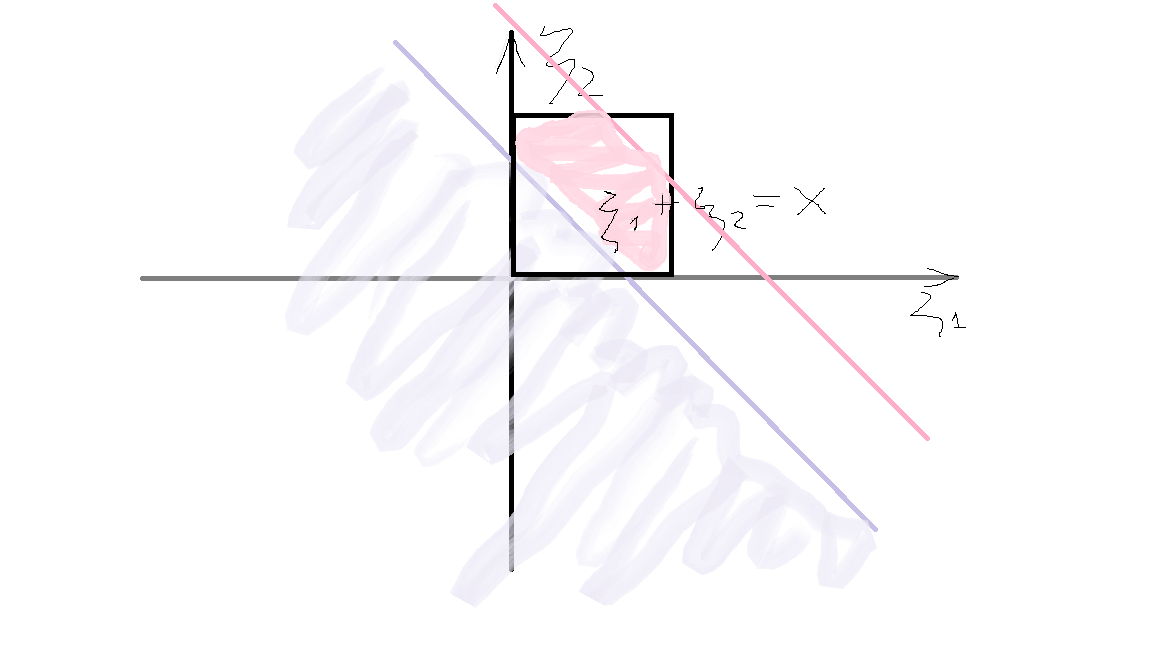
\includegraphics[width=0.7\linewidth]{t24}
\caption{T24}
\label{fig:t24}
\end{figure}

При $x<0$  $ \rho(\xi_1+\xi_2\le x)=0$.

При $x>0$  $ \rho(\xi_1+\xi_2\le x)=1$.

При $ x\in [0,1] $
\[ \rho(\xi_1+\xi_2\le x) =\int_0^x d\xi_1 \int_0^{x-u} d\xi_2= \int_0^x (x-\xi) d\xi= x^2-\frac{x^2}{2}=\frac{x^2}{2} \]

При $ x\in [1,2] $ нужно посчитать площадь, заштрихованную розовым, для этого от площади квадрата отнимем 
оставшуюся площадь, которая легко находится, зная длину сторон этой области.
\[ \rho(\xi_1+\xi_2\le x) =1-\frac{(2-x)^2}{2}=2x-\frac{x^2}{2}-1
\]

В итоге функция распределения имеет вид:
\[ F_{\xi_1+\xi_2}(x)=P(\xi_1 \le x) = 
\begin{cases} 
0,   & \text{если х<0} \\ 
\frac{x^2}{2},  &\text{если }  x\in[0,1) \\
2x-\frac{x^2}{2}-1, &\text{если }  x\in[0,1) \\
1   &\text{если }  x\in[2,+\infty)   
\end{cases}  \]


Найдем плотность распределения:
\[ F_{\xi_1+\xi_2}(x)=P(\xi_1 \le x) = 
\begin{cases} 
0,   & \text{если х<0} \\ 
x^2,  &\text{если }  x\in[0,1) \\
2-x, &\text{если }  x\in[0,1) \\
0  &\text{если }  x\in[2,+\infty)   
\end{cases}  \]



\end{example}


\begin{example}\textbf{T25}

Пусть $\xi_{1}, \xi_{1} -$ независимые случайные величины с распределением Пуассона. 
Найти распределение их суммы и условное распределение $\xi_{1},$ если известна сумма $\xi_{1}+\xi_{2}$


\[ P(\xi_{1}+\xi_{2}=k)=\sum_{i=0}^{k}P(\xi_{1}=i;\xi_2=k-i) \underbrace{=}_{\text{независимость}}
\sum_{i=0}^{k}P(\xi_1=i)P(\xi_2=k-i)= \]
\[ = \sum_{i=0}^{k} \frac{\lambda_1^i \lambda_2^{k-i}}{i! (k-i)!} e^{-\lambda_1-\lambda_2}=
\frac{1}{k!} e^{-\lambda_1-\lambda_2}\sum_{i=0}^{k} C_k^i \lambda_1^i \lambda_2^{k-i}=
\frac{(\lambda_1+\lambda_2)^k}{k!}e^{-(\lambda_1+\lambda_2)}
\]

Теперь найдем 
\[ P(\xi_1=k|\eta =n) =\frac{P(\xi_1=k \cup \xi_2=n-k)}{P(\eta=n)}=
\frac{\xi_1(k)\xi_2(n-k)}{\eta(n)}= C_n^k\frac{(\lambda_1/\lambda_2)^k}{(\lambda_1/\lambda_2+1)^n}\]


\end{example}




\begin{example}\textbf{Т.26.} 

Известно, что случайная величина $\xi$ имеет строго возрастающую непрерывную функцию распределения $F_{\xi}(x) .$ 
Найти распределение случайной величины $\eta=F_{\xi}(\xi) .$


Из непрерывности следует, что $ \exists F^{-1}_\xi (x)$, поэтому просто преобразуем искомую функцию распределения:
\[ F_\eta (x)= 
P(\eta\le x)= P(F_\xi(\xi) \le x) = 
P(\xi\le F^{-1}_\xi (x) )= 
F_\xi(F^{-1}_\xi (x))=x \]
В итоге
\[ F_\eta(x)=
\begin{cases} 
0,   & \text{если х<0} \\ 
x,  & \text{если }  x\in[0,1] \\
1, & x\in[1,+\infty)   
\end{cases}  \]


\end{example}





\begin{example}\textbf{T.27. }


Пусть $\xi$ имеет имеет стандартное нормальное распределение. 
Найти функцию распределения и плотность случайной величины $\xi^{2}$


Функция распределения:
\[ F_{\xi^2}(x)=P(\xi^2\le x)=
P(\xi\le \sqrt{x})=
\frac{1}{\sqrt{2\pi}} e^{-\frac{1}{2} x} \]

А ее плотность находится с помощью производной:
\[ f_{\xi^2}(x)=-\frac{1}{2\sqrt{2\pi}} e^{-\frac{1}{2} x} \]


\end{example}



\begin{example} \textbf{T. 28 }


Пусть $X_{1}, \ldots, X_{n}-$ независимые одинаково распределенные случайные величины с плотностью $f(x) .$ 
Для каждого элементарного события $\omega \in \Omega$ вектор $\left(X_{1}(\omega), \ldots, X_{n}(\omega)\right)$ преобразуем в 
упорядоченный $\left(X_{(1)}(\omega), \ldots, X_{(n)}(\omega)\right),$ 
где $X_{(1)}(\omega) \leq \ldots \leq X_{(n)}(\omega) .$ 
Упорядоченный вектор $\left(X_{(1)}, \ldots, X_{(n)}\right)$ в математической статистике называют вариационным рядом, а случайные величины $X_{(k)}, k=1, \ldots, n-$ порядковыми статистиками. 
Покажите, что плотность совместного распределения порядковых статистик определяется равенством.
$$
f_{X_{(1)}, \ldots, X_{(n)}}\left(x_{1}, \ldots, x_{n}\right)=
n ! f\left(x_{1}\right) \cdot \ldots \cdot f\left(x_{n}\right) \mathbbm{1}_{\left\{x_{1} \leq \ldots \leq x_{n}\right\}}\left(x_{1}, \ldots, x_{n}\right)
$$

Множество, на котором совпали $ X_i, X_j \ i\ne j$ имеет меру ноль.
Для остальных каждому корректному вариационному ряду соответствует $n!$ неупорядоченных векторов.
%
Из независимости $X_1, \ldots X_n$
\[ f_{X_1, X_2, \ldots, X_n}(x_1,x_2,...,x_n)= \prod_{k=1}^n f(x_k) \]
%
Поэтому
$$
f_{X_{(1)}, \ldots, X_{(n)}}\left(x_{1}, \ldots, x_{n}\right)=
n ! f\left(x_{1}\right) \cdot \ldots \cdot f\left(x_{n}\right) \mathbbm{1}_{\left\{x_{1} \leq \ldots \leq x_{n}\right\}}\left(x_{1}, \ldots, x_{n}\right)
$$





\end{example}



\begin{example} \textbf{T. 29 }

Вдоль дороги, длиной в 1 км расположены случайным образом три человека. 
Найти вероятность того, что никакие два человека не находятся друг от друга на расстоянии, меньшем $1 / 4$ км.

Обозначим координаты каждого человека $ x,y,z$. Нужное нам событие $A$ состоит в следующем:
\[  A=
\begin{cases} 
y-x \ge \frac{1}{4} \\ 
z-y \ge \frac{1}{4} \\ 
\frac{1}{4}\le y \le \frac{3}{4}
\end{cases}  \]

\[ P(A)=\int_{\frac{1}{4}}^{\frac{3}{4}} dy \int_{0}^{y-\frac{1}{4}} dx \int_{y+\frac{1}{4}}^{1}dz= 
\int_{\frac{1}{4}}^{\frac{3}{4}} dy \left(y-\frac{1}{4}\right)\left(1-y-\frac{1}{4}\right)=\frac{1}{48}\]

А так как порядок трех точек может быть получен $ 3!=6$ способами, то нужно домножить прошлую вероятность на 6

Ответ: $ P=\frac{1}{8} $

\end{example}







\section{Математическое ожидание и Дисперсия. Ковариация и коэффициент корреляции}


\begin{example} \textbf{T.30.} 

В $N$ ячеек случайно в соответствии со статистикой Бозе-Эйнштейна (частицы неразличимы и размещение без ограничений) размещаются $n$ частиц. Пусть $\xi-$ число пустых ячеек. Найти $\mathrm{E} \xi$ и $\mathrm{D} \xi$.

\[ E \xi = \sum_i E \mathbbm{1}_{A_i}=
\sum_i P(A_i) = N \frac{|A|}{|\Omega|}=
N  \left(1-\frac{1}{N}\right)^n\]

%\frac{C_n^{N+n-2}}{C_n^{N+n-1}}=
%N \frac{(N+n-2)!}{(N+n-1)!}\frac{(N-1)!}{(N-2)!}=\frac{N(N-1)}{N+n-1}

%\[ |A_i A_j (i\ne j)| = C_n^{N+n-3}=\frac{(N+n-3)!}{(N-3)! n!}\]


\[ E\xi^2 = 
E(\sum_{i}\mathbbm{1}_{A_i} +\sum_{i\ne j}\mathbbm{1}_{A_i A_l})=
\sum_{i=k}E \mathbbm{1}_{A_i}^2+\sum_{i\ne k}E \mathbbm{1}_{A_i} \mathbbm{1}_{A_k}=
(N^2-N)\left(1- \frac{2}{N}\right)^n
\]


%N P(A_1)+N(N-1)P(A_1A_2)=
%\frac{N(N+1)}{N+n-1}+\frac{N(N-1)^2(N-2)}{(N+n-1)(N+n-2)}

\[ D\xi = E\xi^2 - (E\xi)^2 =
(N^2-N)\left(1- \frac{2}{N}\right)^n-N^2\left(1-\frac{1}{N}\right)^{2n} \]


\end{example}







\begin{example} \textbf{Т.31.} 


Игральная кость подбрасывается $n$ раз.
Пусть $\xi-$ число появлений единицы, а $\eta-$ число появлений шестёрки. 
Найти коэффициент корреляции этих случайных величин.


Обозначим $ A_i$ - выпадение на i-м броске единицы, $B_i$ - шестерки.
$ \xi =\sum_{i=1}^{n} \mathbbm{1}_{A_i},  \eta = \sum_{i=1}^{n} \mathbbm{1}_{B_i}; $
\[ E \mathbbm{1}_{A_i}= E  \mathbbm{1}_{B_i}=\frac{1}{6} ;  \]
%
\[ \operatorname{cov} (\xi, \eta) =
E(\xi-E\xi) (\eta- E\eta)= E(\xi\eta)-E\xi E\eta\]

\[ E(\xi\eta)=E(\sum_{i=1}^{n}\mathbbm{1}_{A_i}) (\sum_{k=1}^{n}\mathbbm{1}_{B_k})= E(\sum_{i=1}^{n}\mathbbm{1}_{A_i}\mathbbm{1}_{B_i})+E(\sum_{i\ne k} \mathbbm{1}_{A_i} \mathbbm{1}_{B_k}) =\sum_{i\ne k} E \mathbbm{1}_{A_i} \mathbbm{1}_{B_k}=\frac{n(n-1)}{36} \]

\[ \operatorname{cov}(\xi,\eta)=
\frac{n(n-1)}{36}-\frac{n^2}{36}=-\frac{n}{36}  \]


\[ D\xi =\sum_{i=1}^{n} D \mathbbm{1}_{A_i} = \sum_{i=1}^{n}(E \mathbbm{1}_{A_i}^2- (E\mathbbm{1}_{A_i})^2 ) =
n\left(\frac{1}{6}-\frac{1}{6}\frac{1}{6}\right) = \frac{5}{36}n\]
\[ D \eta =\frac{5n}{36} \]

\[ \operatorname{cov}(\xi,\eta)=\dfrac{-\frac{n}{36}}{\frac{5n}{36}}=-\frac{1}{5} \]


\end{example}



\begin{example} \textbf{Т.32.} 

Подбрасывают две игральные кости. 
Пусть $\xi_{1}-$ число очков на первой игральной кости, а $\xi_{2}-$ на второй. 
Определим $\eta_{1}=\xi_{1}+\xi_{2}$ $\eta_{2}=\xi_{1}-\xi_{2} .$ 
Найти $\operatorname{cov}\left(\eta_{1},\eta_{2}\right)$ и выяснить, являются ли $\eta_{1}$ и $\eta_{2}$ независимыми.



\[ \operatorname{cov}(\eta_{1},\eta_{2})=
E(\eta_{1},\eta_{2})-E(\eta_{1}) E(\eta_{2}) =
E(\eta_{1}^2)- E(\eta_{2}^2)-(E\eta_{1})^2
+(E\eta_{2})^2= D\eta_{1} - D \eta_{2}= 0\]

Зависимость следует из контрпримера.
Из подсчета количества благоприятных успехов, видим, что
\[ P(\eta_1=2)=\frac{1}{36}; P(\eta_2 =0) = \frac{1}{6} \]
и в то же время
\[ P(\eta_{1}=1, \eta_{2}=0)=P (\eta_{1}=1, \eta_{2}=1)= \frac{1}{36} \]


\end{example}



\begin{example}\textbf{T.33. }


Доказать, что если случайные величины $\xi$ и $\eta$ принимают только
по два значения каждая, то из некоррелируемости следует их независимость.


$ \xi\in \{a_1, a_2\}; \eta \in \{b_1, b_2\}$,
\[ \operatorname{cov}(\xi,\eta)= E\xi\eta -E\xi E\eta=0 \]
\[ E\xi\eta =\sum_{i,k=1}^{2}a_ib_k E(\mathbbm{1}_{A_i} \mathbbm{1}_{B_k})=
\sum_{i,k=1}^{2} a_ib_k P(A_i, B_k)
\]
\[ E\xi E\eta = (
\sum_{i=1}^{2} a_i P(A_i))
(\sum_{k=1}^{2} b_k P( B_k))=
\sum_{i,k=1}^{2} a_ib_k P(A_i P(B_k) \]
Поэтому 
\[ \operatorname{cov}(\xi,\eta)=0=
\sum_{i,k=1}^{2} a_ib_k (P(A_i, B_k)-P(A_i)P(B_k)) \rightarrow P(A_iB_k)=P(A-i)P(B_k)\]


\end{example}





\begin{example} \textbf{Т.34. }


Авария происходит в точке $X,$ которая равномерно распределена на дороге длиной $L .$ 
Во время аварии машина скорой помощи находится в точке $Y$, которая также равномерно распределена на дороге. 
Считая, что $X$ и $Y$ независимы, найдите математическое ожидание расстояния между машиной скорой помощи и точкой аварии.


\[ E|X-Y|= \int_{[0,L]^2} |x-y| \rho_X (x) \rho_Y(y) dx dy = 
\int_{[0,L]^2} \frac{|x-y|}{L^2} dx dy=\frac{2}{L}\int_0^L dx \int_{x}^{L} (y-x) dy =\frac{2}{L}\frac{L^3}{6} =\frac{L}{3} \]








\end{example}














\clearpage
\part{Второе задание}






\section{Неравенства Чебышева и Маркова. Законы больших чисел}










\begin{example}\textbf{T 1}

Известно, что число посетителей некоторого салона в день является случайной величиной со средним значением $50 .$

(a) Оценить вероятность того, что число посетителей в конкретный день превысит 75


так как

$$
\mathbf{P}\{|\xi| \geqslant x\} \leqslant \frac{\mathbf{M}|\xi|}{x}
$$

то


$$
P(\xi \geq 75) \leq \frac{50}{75}=\frac{2}{3}
$$



(b) При условии, что дисперсия числа посетителей в день равна $25,$ 
оценить вероятность того, что в конкретный день их число будет между 40 и $60 .$


$$
P(|\xi-50| \geq 10) \leq \frac{25}{100}=\frac{1}{4} 
$$

поэтому

\[  
P(|\xi-50|<10)=1-P(|\xi-50| \geq 10) \geq \frac{3}{4} 
\]




\end{example}



\begin{example} T. 2. 


$\mathrm{C}$ помошью неравенства Чебышева оценить вероятность того, что при 1000 бросаниях монеты число выпадений герба окажется в промежутке [450,550]





Дисперсия в таком эксперименте
$$
E\xi^2)=E(\sum_{i}^{n}1_{A_i})+E(\sum_{i\ne j}^{n})=500+(1000^2-100)/4=
$$



\[ D(\xi)=E(\xi^2)-(E(\xi))^2=250 \]

Неравенство Чебышева даст:
$$
P(|\xi-500| \geq 50) \leq \frac{250}{500}  $$



\[ P(|\xi-500|<50)=1-P(|\xi-500| \geq 50) \geq
0.9
 \]




\end{example}



\begin{example} T.3. 


Вероятность того, что изделие качественное, равна $0,9 .$ 
Каков должен быть объем партии изделий, чтобы с вероятностью $\geq 0,95$ можно было утверждать, что отклонение (по абсолютной величине) доли качествен-
ных изделий от 0,9 не превысит $0,01 ?$




\[ P(|\xi-0,9|<0,01)=1-P(|\xi-0,9| \geq 0,01) \geq 0,95 \rightarrow P(|\xi-0,9| \geq 0,01) \leq 0,05=\frac{\sigma(\xi)^{2}}{10^{-4}}  \]


но также 
$  \sigma(\xi)=\sqrt{D(\xi)}=\frac{1}{n} \sqrt{n \cdot 0,9 \cdot 0,1}=\frac{0,3}{\sqrt{n}},$
поэтому:

\[ 
0,05=\frac{0,3^{2}}{n \cdot 10^{-4}} \rightarrow n=\frac{0,3^{2}}{0,05 \cdot 10^{-4}}=18000
\]








\end{example}





\begin{example} T.4. (Одностороннее неравенство Чебышева.) 


Пусть случайная величина $\xi$ имеет нулевое среднее и дисперсию $\sigma^{2}$. 
Показать, что для $\varepsilon>0$ выполняется неравенство
$$
P(\xi \geq \varepsilon) \leq \frac{\sigma^{2}}{\sigma^{2}+\varepsilon^{2}}
$$



Очевидно, что для $b>0$
$$
P(\xi \geq \epsilon) \leq P\left((\xi+b)^{2} \geq(\epsilon+b)^{2}\right) \leq \frac{\mathbb{E}\left((\xi+b)^{2}\right)}{(\epsilon+b)^{2}}=\frac{\mathbb{E}\left(\xi^{2}+2 \xi b+b^{2}\right)}{(\epsilon+b)^{2}}=\frac{\mathbb{E}\left(\xi^{2}\right)+b^{2}}{(\epsilon+b)^{2}}
$$
Правая часть имеет минимум при $b=\frac{\sigma^{2}}{\epsilon} .$ Подставляя это значение, приходим к нужному неравенству.







\end{example}







\begin{example} T. 5. $($ Неравенство Иенсена. $)$ 

Пусть $\varphi:(a, b) \rightarrow \mathbb{R}-$ дважды непрерывно дифференцируемая функция и $\varphi^{\prime \prime}(x) \geq 0$ для всех $x \in(a, b)$ (т. е. $\varphi$ Выпуклая функция, и допускается $a=-\infty$ и $b=\infty$ ). 
Допустим также, что $\xi-$ случайная величина, которая принимает значения из $(a, b)$ и $\mathrm{E} \xi=m, \mathrm{E} \varphi(\xi)$ конечны. Показать, что тогда
$$
\mathrm{E} \varphi(\xi) \geq \varphi(\mathrm{E} \xi)=\varphi(m)
$$



$$
\varphi(x) \geq \varphi^\prime \left(x_{0}\right)\left(x-x_{0}\right)+\varphi\left(x_{0}\right)
$$
Пусть
$$
\varphi(\xi) \geq \lambda(\mathbb{E}(\xi))(\xi-\mathbb{E}(\xi))+\varphi(\mathbb{E}(\xi))
$$
Берём матожидание ои обеих частей.
$$
\mathbb{E}(\varphi(\xi)) \geq \lambda(\mathbb{E}(\xi))(\mathbb{E}(\xi)-\mathbb{E}(\xi))+\mathbb{E}(\varphi(\mathbb{E}(\xi)))=
\varphi(\mathbb{E}(\xi))
$$






\end{example}



\begin{example}



T.6. 


Пусть $\xi-$ слу чайная величина, имеющая нормальное распределение с параметрами $\left(a, \sigma^{2}\right) .$ Показать, что для $\varepsilon>0$ выполняется неравенство

$$
\mathrm{P}(|\xi-a| \geq \varepsilon \sigma) \leq \frac{1}{\varepsilon} \sqrt{\frac{2}{\pi}} e^{-\varepsilon^{2} / 2}
$$



\[ \begin{aligned}
P(|\xi| \geq \epsilon \sigma)
=
\left(\int_{\epsilon \sigma}^{+\infty}
+
\int_{-\infty}^{-\epsilon \sigma}\right) 
\frac{1}{\sqrt{2 \pi} \sigma} 
\exp \left(-\frac{x^{2}}{2 \sigma^{2}}\right) d(x) 
&=
\int_{\epsilon \sigma}^{+\infty} \frac{\sqrt{2}}{\sqrt{\pi} \sigma} \exp \left(-\frac{x^{2}}{2 \sigma^{2}}\right) d(x)
=
\\
=& \sqrt{\frac{2}{\pi}} \int_{\epsilon}^{+\infty} 
\exp \left(-\frac{x^{2}}{2}\right) d(x) 
\leq 
\sqrt{\frac{2}{\pi}} \frac{1}{\epsilon} 
\exp \left(-\frac{\epsilon^{2}}{2}\right)
\end{aligned} \]






\end{example}



\begin{example}

T.7. Пусть $\xi_{1}, \xi_{2}, \ldots$ - последовательность одинаково распределенных сл учайных величин такая, что $\mathrm{E} \xi_{k}=a, \mathrm{D} \xi_{k}=\sigma^{2}$ и $\operatorname{cov}\left(\xi_{i}, \xi_{j}\right)=(-1)^{i-j} v$
$i \neq j .$ 
Доказать, что для всякого $\varepsilon>0$ выполняется предельное соотношение
$$
\lim _{n \rightarrow \infty} \mathrm{P}\left(\left|\frac{1}{n} \sum_{k=1}^{n} \xi_{k}-a\right| \geq \varepsilon\right)=0
$$













\end{example}





\begin{example} T.8. 

Пусть $\left\{\xi_{n}\right\}-$ последовательность неотрицательных случайных величин с конечными математическими ожиданиями и $\xi_{n} \stackrel{\text { п.н. }}{\rightarrow} \xi, \mathrm{E} \xi<\infty$ $\mathrm{E} \xi_{n} \rightarrow \mathrm{E} \xi$ при $n \rightarrow \infty .$ 

Покажите, что тогда $\mathrm{E}\left|\xi_{n}-\xi\right| \rightarrow 0$ при $n \rightarrow \infty$
T. e. $\xi n \stackrel{L}{\rightarrow} \xi$




$\forall n \in \mathbb{N}:$
$$
\left|\mathbb{E}\left(\xi_{n}\right)\right|<+\infty,|\mathbb{E}(\xi)|<+\infty \rightarrow \mathbb{E}\left|\xi_{n}-\xi\right|<+\infty
$$
$\forall \epsilon>0:$
$$
\begin{array}{l}
\mathbb{E}\left|\xi_{n}-\xi\right|=\mathbb{E}\left|\left(\xi_{n}-\xi\right)\left(I\left(\sup _{k \geq n}\left(\left|\xi_{k}-\xi\right|>\epsilon\right)\right)+I\left(\sup _{k \geq n}\left(\left|\xi_{k}-\xi\right| \leq \epsilon\right)\right)\right)\right|= 
\\
=\mathbb{E}\left|\left(\xi_{n}-\xi\right) I\left(\sup _{k \geq n}\left(\left|\xi_{k}-\xi\right|>\epsilon\right)\right)\right|+\mathbb{E}\left|\left(\xi_{n}-\xi\right) I\left(\sup _{k \geq n}\left(\left|\xi_{k}-\xi\right| \leq \epsilon\right)\right)\right|
\end{array}
$$
Первый индикатор в пределе принимает значение 1 только на множестве меры 0. Второй индикатор в пределе принимает значение 1 почти всюду. Но тогда под вторым математическим ожиданием стоит выражение $\left|\xi_{k}-\xi\right| \leq \epsilon$. $\Rightarrow \mathbb{E}\left|\xi_{k}-\xi\right| \leq \mathbb{E}(\epsilon)=\epsilon$









\end{example}














\section{ Метод характеристических функций. Центральная предельная теорема}



\begin{example} Т.9. 

Найти характеристическую функцию распределения Лапласа, которое определяется плотностью
$$
f_{\xi}(x)=\frac{1}{2} e^{-|x|}
$$





\[ 	\phi_{\xi}(t)=\int_{-\infty}^{+\infty} \exp (i t x) f_{\xi}(x) d(x)=\frac{1}{2} \int_{-\infty}^{+\infty} \exp (i t x-|x|) d(x) \]



$ x<0$


\[ \int_{-\infty}^{0} \exp (i t x-|x|) d(x)=\int_{-\infty}^{0} \exp (i t x+x) d(x)=\frac{i}{i-t} \]


$ x \geq 0 $



\[ \int_{0}^{+\infty} \exp (i t x-|x|) d(x)=\int_{0}^{+\infty} \exp (i t x-x) d(x)=\frac{i}{i+t} \]



\[ \phi_{\xi}(t)=\frac{-1}{\left(-1-t^{2}\right)}=\frac{1}{1+t^{2}} \]










\end{example}



\begin{example} T.10. 


Найти характеристическую функцию нормального распределения с параметрами $\left(a, \sigma^{2}\right)$





\begin{equation}
\begin{array}{l}
\phi_{\xi}(t)=\int_{-\infty}^{+\infty} \exp (i t x) \frac{1}{\sqrt{2 \pi \sigma^{2}}} \exp \left(-\frac{(x-a)^{2}}{2 \sigma^{2}}\right) d(x)=\frac{1}{\sqrt{2 \pi \sigma^{2}}} \int_{-\infty}^{+\infty} \exp \left(i t x-\frac{(x-a)^{2}}{2 \sigma^{2}}\right) d(x)= \\
\begin{array}{c}
1 \\
=\frac{1}{\sqrt{2 \pi \sigma^{2}}} \exp \left(i t a+\left(\frac{i t \sqrt{2} \sigma}{2}\right)^{2}\right) \int_{-\infty}^{+\infty} \exp \left(-\frac{(x-a)^{2}}{2 \sigma^{2}}+2 \frac{i t \sqrt{2} \sigma}{2} \frac{(x-a)}{\sqrt{2} \sigma}-\left(\frac{i t \sqrt{2} \sigma}{2}\right)^{2}\right) d(x)= \\
\frac{1}{\sqrt{2 \pi \sigma^{2}}} \exp \left(i t a+\left(\frac{i t \sqrt{2} \sigma}{2}\right)^{2}\right) \int_{-\infty}^{+\infty} \exp \left(-\left(\frac{x-a}{\sqrt{2} \sigma}-\frac{i t \sqrt{2} \sigma}{2}\right)^{2}\right) d(x)= \\
=\frac{1}{\sqrt{2 \pi \sigma^{2}}} \exp \left(i t a+\left(\frac{i t \sqrt{2} \sigma}{2}\right)^{2}\right) \int_{-\infty}^{+\infty} \exp \left(-\left(\frac{x-a-i t \sigma^{2}}{\sqrt{2} \sigma}\right)^{2}\right) d(x)=\frac{1}{\sqrt{2 \sigma^{2}}} \exp \left(i t a-\frac{t^{2} \sigma^{2}}{2}\right)
\end{array}
\end{array}
\end{equation}









\end{example}



\begin{example}

Т.11. Найти распределения, которым соответствуют следуюшие характеристические функции:
$$
h_{1}(t)=\cos t ; 
\quad 
h_{2}(t)=\frac{1}{2}+\frac{\cos t}{2}+i \frac{\sin t}{6} ; 
\quad 
h_{3}(t)=\frac{1}{2-e^{-i t}}
$$


для первой:


\begin{equation}
h_{1}(t)=\cos (t)=\frac{\exp (i t)+\exp (-i t)}{2} \rightarrow f_{1}(x)=\frac{1}{2} I(x=1)+\frac{1}{2} I(x=-1)
\end{equation}





Для второй:

$$
h_{2}(t)=\frac{1}{2}+\frac{\cos (t)}{2}+i \frac{\sin (t)}{6}=
$$


$$
=
\frac{1}{2} \exp (i t \cdot 0)+\frac{\exp (i t)+\exp (-i t)}{4}+i \frac{\exp (i t)-\exp (-i t)}{12}
=
$$


$$
=
\frac{1}{2} \exp (i t \cdot 0)+\frac{\exp (i t)+\exp (-i t)}{4}+i \frac{\exp (i t)-\exp (-i t)}{12}
$$

поэтому

$$
f_{2}(x)=\frac{1}{2} \delta(x)+\frac{1}{4} \delta(x-1)+\frac{1}{4} \delta(x+1)+i \frac{1}{12} \delta(x-1)-i \frac{1}{12} \delta(x+1)
$$



для третьей:


$$
h_{3}(t)=\frac{1}{2-\exp (-i t)}=\frac{\frac{1}{2}}{1-\frac{\exp (-i t)}{2}}=\sum_{n=0}^{+\infty}\left(\frac{\exp (i t n)}{2^{n+1}}\right)
$$


\[ f_{3}(x)=\sum_{n=0}^{+\infty}\left(\frac{1}{2^{n+1}} I(x=n)\right)
 \]






\end{example}





\begin{example} T.12. 

Найти распределение, которому соответствует характеристическая функция $h(t)=e^{-t^{2}} \cos t$



$$
h(t)=\exp \left(-t^{2}\right) \cos (t) \rightarrow f(x)=\int_{-\infty}^{+\infty} \exp \left(-t^{2}\right) \cos (t) \exp (-i t x) d(t)=
$$


$$
=\int_{-\infty}^{+\infty} \frac{\exp \left(-t^{2}-i t x+i t\right)+\exp \left(-t^{2}-i t x-i t\right)}{2} d(t)
=
$$


\[ \int_{-\infty}^{+\infty} \frac{\exp \left(-t^{2}-i t(x-1)\right)+\exp \left(-t^{2}-i t(x+1)\right)}{2} d(t)=
\]



$$
=\int_{-\infty}^{+\infty}
\frac{ 
	\exp \left(-t^{2}-2 t \frac{x-1}{2} i-\left(\frac{x-1}{2} i\right)^{2}
	+\left(\frac{x-1}{2} i\right)^{2}\right)
	+
	\exp \left(-t^{2}-2 t \frac{x+1}{2} i-\left(\frac{x+1}{2} i\right)^{2}+\left(\frac{x+1}{2} i\right)^{2}\right)
}{2} d(t)=
$$


$$
=\int_{-\infty}^{+\infty} \frac{\exp \left(-\left(t+\frac{x-1}{2} i\right)^{2}+\left(\frac{x-1}{2} i\right)^{2}\right)+\exp \left(-\left(t+\frac{x+1}{2} i\right)^{2}+\left(\frac{x+1}{2} i\right)^{2}\right)}{2} d(t)=
$$




$$
=\int_{-\infty}^{+\infty} \frac{\exp \left(-\left(t+\frac{x-1}{2} i\right)^{2}\right) \exp \left(\left(\frac{x-1}{2} i\right)^{2}\right)+\exp \left(-\left(t+\frac{x+1}{2} i\right)^{2}\right) \exp \left(\left(\frac{x+1}{2} i\right)^{2}\right)}{2} d(t)=
$$




$$
=\sqrt{\pi} \frac{\exp \left(-\left(\frac{x-1}{2}\right)^{2}\right)+\exp \left(-\left(\frac{x+1}{2}\right)^{2}\right)}{2}
$$



Вот такому распределению.




\end{example}







\begin{example} \textbf{Т.13 }

Является ли функция $h(t)=\cos t^{2}$ характеристической?



$\cos \left(t^{2}\right)$ не является равномерно непрерывной на $\mathbb{R}$, а следовательно, и не может быть характеристической функцией.

Докажем это.


Нужно доказать, что


\[ \exists \epsilon>0: \forall \delta>0 
\exists t_{1}, t_{2}\left|t_{2}-t_{1}\right|<\delta 
\Rightarrow\left|\cos \left(t_{2}^{2}\right)-\cos \left(t_{1}^{2}\right)\right| \geq \epsilon \]



Найлём решения уравнения $\cos \left(t^{2}\right)=1:$
$$
t^{2}=2 \pi n, n \in \mathbb{N} \cup\{0\}
$$
Найдём решения уравнения $\cos \left(t^{2}\right)=-1:$

\[ t^{2}=2 \pi n-\pi, n \in \mathbb{N} \]


$$
\text { Пусть } t_{1}=\sqrt{2 \pi n}, t_{2}=\sqrt{2 \pi n-\pi .} \text { Тогда }\left|\cos \left(t_{2}^{2}\right)-\cos \left(t_{1}^{2}\right)\right|=2=\epsilon
$$


\[ \left|t_{2}-t_{1}\right|
=
|\sqrt{2 \pi n}-\sqrt{2 \pi n-\pi}|
=
\frac{\pi}{\sqrt{2 \pi n}+\sqrt{2 \pi n-\pi}}
<
\sqrt{\frac{\pi}{n}} 
\Rightarrow 
n>\frac{\pi}{\delta^{2}} \Rightarrow \]



\[ \exists \epsilon=2: \forall \delta>0 \exists t_{1}=\sqrt{2 \pi n}, t_{2}
=
\sqrt{2 \pi n-\pi}, n>\frac{\pi}{\delta^{2}},\left|t_{2}-t_{1}\right|
<
\delta 
\Rightarrow
\left|\cos \left(t_{2}^{2}\right)-\cos \left(t_{1}^{2}\right)\right| 
\geq \epsilon \]


Доказали.




\end{example}



\begin{example} Т.14. 

Случайная величина $\xi_{\lambda}$ распределена по закону Пуассона с параметром $\lambda .$ Найти
$$
\lim _{\lambda \rightarrow \infty} \mathrm{P}\left(\frac{\xi_{\lambda}-\lambda}{\sqrt{\lambda}} \leqslant x\right)
$$



$$
\text { Рассмотрим, к чему стремится характеристическая функция случайной величины } \eta=\frac{\xi_{\lambda}-\lambda}{\sqrt{\lambda}}
$$


$$
\phi_{\eta}(t)=\mathbb{E}\left(\exp \left(i t \frac{\xi_{\lambda}-\lambda}{\sqrt{\lambda}}\right)\right)=\exp (-i t \sqrt{\lambda}) \mathbb{E}\left(\exp \left(i t \frac{\xi_{\lambda}}{\sqrt{\lambda}}\right)\right)=
$$


$$
=\exp (-i t \sqrt{\lambda}) \exp \left(\lambda\left(\exp \left(\frac{i t}{\sqrt{\lambda}}\right)-1\right)\right)=\exp \left(-i t \sqrt{\lambda}+\lambda\left(\exp \left(\frac{i t}{\sqrt{\lambda}}\right)-1\right)\right)
$$


$$
\lim _{\lambda \rightarrow+\infty}\phi_{\eta}(t)
=
\lim _{\lambda \rightarrow+\infty}
\exp \left(-i t \sqrt{\lambda}+\lambda\left(\exp \left(\frac{i t}{\sqrt{\lambda}}\right)-1\right)\right)=
$$


$$
=\lim _{\lambda \rightarrow+\infty}\exp \left(-i t \sqrt{\lambda}+\lambda\left(1+\frac{i t}{\sqrt{\lambda}}+\frac{1}{2}\left(\frac{i t}{\sqrt{\lambda}}\right)^{2}+o\left(\left(\frac{t}{\sqrt{\lambda}}\right)^{2}\right)-1\right)\right)=
$$


$$
=\lim _{\lambda \rightarrow+\infty}\exp \left(-i t \sqrt{\lambda}+\lambda\left(\frac{i t}{\sqrt{\lambda}}-\frac{1}{2} \frac{1}{\lambda} t^{2}+o\left(\left(\frac{t}{\sqrt{\lambda}}\right)^{2}\right)\right)\right)
$$



$$
=\lim _{\lambda \rightarrow+\infty}
\exp \left(-\frac{1}{2} t^{2}+o\left(\left(\frac{t}{\sqrt{\lambda}}\right)^{2}\right)\right)
=
\exp \left(-\frac{1}{2} t^{2}\right)
$$


$$
\lim _{\lambda \rightarrow+\infty}\left(P\left(\frac{\xi_{\lambda}-\lambda}{\sqrt{\lambda}} \leq x\right)\right)=\int_{-\infty}^{x} \exp \left(-\frac{1}{2} t^{2}\right) d(t)=\Phi(x)
$$








\end{example}



\begin{example} T. 15. 

Используя результат предыдущей задачи, найти предел
$$
\lim _{n \rightarrow \infty} e^{-n} \sum_{k=n}^{n} \frac{n^{k}}{k !}
$$



Так как
$$
\Phi(x)=\lim _{\lambda \rightarrow+\infty}
P\left(\frac{\xi_{\lambda}-\lambda}{\sqrt{\lambda}} \leq x\right)
=
\lim _{\lambda \rightarrow+\infty}
P\left(\xi_{\lambda} \leq \sqrt{\lambda} x+\lambda\right)=
$$



\[ =\lim _{\lambda \rightarrow+\infty}\left[\exp (-\lambda) \sum_{k=1}^{\lfloor\sqrt{\lambda} x+\lambda\rfloor}\left(\frac{\lambda^{k}}{(k) !}\right)\right]
=
\lim _{\lambda \rightarrow+\infty}
\left[
\exp (-\lambda)\left(
\sum_{k=1}^{\lfloor\lambda\rfloor}
\frac{\lambda^{k}}{(k) !}
+
\sum_{k=\lfloor\lambda\rfloor+1}^{\lfloor\sqrt{\lambda} x+\lambda\rfloor}
\frac{\lambda^{k}}{(k) !}
\right)\right] \]



Теперь рассмотрим случай $\lambda \in \mathbb{N}$ :

$$
\Phi(x)=\lim_{n \rightarrow+\infty}\left(
e^{-n}\left(\sum_{k=1}^{n}\left(\frac{n^{k}}{(k) !}\right)
+
\sum_{k=n+1}^{\lfloor\sqrt{n} x+n\rfloor}\frac{n^{k}}{(k) !}\right)
\right) 
$$


\[ 
\Phi(x)=
\lim _{n \rightarrow+\infty}\left[\exp (-n) \sum_{k=n+1}^{\lfloor\sqrt{n} x+n\rfloor}\left(\frac{n^{k}}{(k) !}\right)\right]
+
\lim _{n \rightarrow+\infty}\left[
\exp (-n) \sum_{k=1}^{n}\left(\frac{n^{k}}{(k) !}\right)
\right] \]



Возьмём теперь предел $x \rightarrow+\infty$ :
$$
\Phi(+\infty)=1=\lim_{n \rightarrow+\infty}\left(\exp (-n) \sum_{k=1}^{n}\left(\frac{n^{k}}{(k) !}\right)\right)
$$









\end{example}





\begin{example} \textbf{Т.16.} 

Пусть положительные независимые случайные величины $\xi_{m, n}$ $m=1,2, \ldots, n$ одинаково распределены с плотностью $\alpha_{n} e^{-\alpha_{n} x}, x>0,$ где $\alpha_{n}=\lambda n$ и $\lambda>0 .$ Найти предельное при $n \rightarrow \infty$ распределение случайной величины $\xi_{n}=\sum_{m=1}^{n} \xi_{m, n}$



$$
f(x)=\alpha_{n} \exp \left(-\alpha_{n} x\right)=\lambda n \exp (-\lambda n x)
$$
Найдём характеристическую функцию случайной величины $\xi_{m, n}:$
$$
\phi_{\xi_{m, n}}(t)=\mathbb{E}(\exp (i t x))=\int_{\mathbb{R}^{+}} \lambda n \exp (-\lambda n x) \exp (i t x) d(x)=\lambda n \int_{\mathbb{R}^{+}} \exp (-\lambda n x) \exp (i t x) d(x)=
$$



\[ \int_{\mathbb{R}^{+}} \lambda n \exp (-\lambda n x) \exp (i t x) d(x)=-\int_{\mathbb{R}^{+}} \frac{\partial}{\partial(x)}(\exp (-\lambda n x)) \exp (i t x) d(x)= \]


\[ =i t \int_{\mathbb{R}^{+}} \exp (-\lambda n x) \exp (i t x) d(x)-\left.(\exp (-\lambda n x) \exp (i t x))\right|_{x=0} ^{x \rightarrow+\infty}=i t \int_{\mathbb{R}^{+}} \exp (-\lambda n x) \exp (i t x) d(x)+1 \rightarrow \]



\[ \rightarrow \phi_{\xi_{m, n}}(t)=\int_{\mathbb{R}^{+}} \lambda n \exp (-\lambda n x) \exp (i t x) d(x)=\frac{\lambda n}{\lambda n-i t}=1-\frac{i t}{i t-\lambda n} \]



Найдём предел характеристических функций:
$$
\phi(t)=\lim _{n \rightarrow+\infty}\left(\phi_{\sum_{m=1}^{n}\left(\xi_{m, n}\right)}(t)\right)=\lim _{n \rightarrow+\infty}\left(\left(1-\frac{1}{1-\frac{\lambda n}{i t}}\right)^{n}\right)=\lim _{n \rightarrow+\infty}\left(\exp \left(n \ln \left(1-\frac{1}{1-\frac{\lambda n}{i t}}\right)\right)\right)
$$



\[ =\lim _{n \rightarrow+\infty}\left(\exp \left(-\frac{1}{\frac{1}{n}-\frac{\lambda}{i t}}\right)\right)=\exp \left(\frac{i t}{\lambda}\right)  \]



\[ f(x)=I\left(x=\frac{1}{\lambda}\right) \]




\end{example}


















\section{Элементы теории случайных процессов и математической статистики}




\begin{example} T. $17 .$ 

Население региона делится по некоторому социально-экономическому признаку на три подгруппы. Следующее поколение с вероятностями 0,$4 ; 0,6$ и $0,2,$ соответственно, остается в своей подгруппе, а если не
Остается, то с равным и вероятностями переходит в Любую из остальных подгрупп. Найти:

a) распределение населения по данному социально-экономическому 
признаку в следующем поколении, если в настоящем поколении в 1 -ой подгруппе было $20 \%$ населения, во 2 -ой подгруппе $-30 \%,$ и в 3 -ей подгруппе $-50 \%$




Данный процесс описывается марковской цепью с матрицей
$$
\left(\begin{array}{lll}
0,4 & 0,3 & 0,3 \\
0,2 & 0,6 & 0,2 \\
0,4 & 0,4 & 0,2
\end{array}\right)
$$
По условию начальное распределение было $(0,2 \quad 0,3 \quad 0,5)$. Тогда распределение в следующем поколении
$$
\left(\begin{array}{lllll}
x & y & z
\end{array}\right)=\left(\begin{array}{lll}
0,2 & 0,3 & 0,5
\end{array}\right)\left(\begin{array}{lll}
0,4 & 0,3 & 0,3 \\
0,2 & 0,6 & 0,2 \\
0,4 & 0,4 & 0,2
\end{array}\right)=\left(\begin{array}{lll}
0,34 & 0,44 & 0,22
\end{array}\right)
$$



Найти б) предельное распределение по данному признаку, которое не меняется при смене поколений.





$$
\left(\begin{array}{ccc}
0,4-\lambda & 0,3 & 0,3 \\
0,2 & 0,6-\lambda & 0,2 \\
0,4 & 0,4 & 0,2-\lambda
\end{array}\right)\left(\begin{array}{l}
x \\
y \\
z
\end{array}\right)=\left(\begin{array}{l}
0 \\
0 \\
0
\end{array}\right) \rightarrow \lambda^{3}-1,2 \lambda^{2}+0,18 \lambda+0,02=0
$$



$$
\lambda_{1}=1, \lambda_{2}=\frac{1+\sqrt{3}}{10}, \lambda_{3}=\frac{1-\sqrt{3}}{10}
$$



$$
\left(\begin{array}{ccc}
0,4-\lambda_{1} & 0,3 & 0,3 \\
0,2 & 0,6-\lambda_{1} & 0,2 \\
0,4 & 0,4 & 0,2-\lambda_{1}
\end{array}\right)\left(\begin{array}{l}
x_{1} \\
y_{1} \\
z_{1}
\end{array}\right)=\left(\begin{array}{l}
0 \\
0 \\
0
\end{array}\right) 
$$


\[ 
\left(\begin{array}{ccc}
	-2 x_{1} & y_{1} & z_{1} \\
	x_{1} & -2 y_{1} & z_{1} \\
	x_{1} & y_{1} & -2 z_{1}
\end{array}\right)=\left(\begin{array}{l}
	0 \\
	0 \\
	0
\end{array}\right)  
\]


\[ 
\left(\begin{array}{l}
	x_{1} \\
	y_{1} \\
	z_{1}
\end{array}\right)
=
\left(\begin{array}{l}
	1 \\
	1 \\
	1
\end{array}\right) 
\]


Аналогично получаем:

$$
\left(\begin{array}{l}
x_{2} \\
y_{2} \\
z_{2}
\end{array}\right)=\left(\begin{array}{c}
\frac{3}{4}(1+\sqrt{3}) \\
\frac{1}{2}(-2-\sqrt{3}) \\
1
\end{array}\right)
$$

$$
\left(\begin{array}{l}
x_{3} \\
y_{3} \\
z_{3}
\end{array}\right)=\left(\begin{array}{c}
\frac{3}{4}(1-\sqrt{3}) \\
\frac{1}{2}(-2+\sqrt{3}) \\
1
\end{array}\right)
$$



Тогда диагонализованная матрица $$\left(\begin{array}{ccc}1 & 0 & 0 \\ 0 & \frac{1+\sqrt{3}}{10} & 0 \\ 0 & 0 & \frac{1-\sqrt{3}}{10}\end{array}\right)$$

и

$$
  \resizebox{\hsize}{!}{%
	$
	\left(\begin{array}{ccc}0,4 & 0,3 & 0,3 \\ 0,2 & 0,6 & 0,2 \\ 0,4 & 0,4 & 0,2\end{array}\right)^{n}
=
\left(\begin{array}{ccc}
	1 & \frac{3}{4}(1+\sqrt{3}) & \frac{3}{4}(1-\sqrt{3}) \\ 
	1 & \frac{1}{2}(-2-\sqrt{3}) & \frac{1}{2}(-2+\sqrt{3}) \\ 
	1 & 1 & 1
\end{array}\right)
\left(\begin{array}{ccc}
	1 & 0 & 0 \\ 
	0 & \frac{1+\sqrt{3}}{10} & 0 \\ 
	0 & 0 & 
	\frac{1-\sqrt{3}}{10}
\end{array}\right)^{n}
\left(\begin{array}{ccc}
1 & \frac{3}{4}(1+\sqrt{3}) & \frac{3}{4}(1-\sqrt{3}) \\ 
1 & \frac{1}{2}(-2-\sqrt{3}) & \frac{1}{2}(-2+\sqrt{3}) \\ 
1 & 1 & 1
\end{array}\right)^{-1}=
$}
$$



\[ 
=\left(\begin{array}{ccc}
1 & \frac{3}{4}(1+\sqrt{3}) & \frac{3}{4}(1-\sqrt{3}) \\
1 & \frac{1}{2}(-2-\sqrt{3}) & \frac{1}{2}(-2+\sqrt{3}) \\
1 & 1 & 1
\end{array}\right)
\left(\begin{array}{ccc}
1 & 0 & 0 \\
0 & \left(\frac{1+\sqrt{3}}{10}\right)^{n} & 0 \\
0 & 0 & \left(\frac{1-\sqrt{3}}{10}\right)^n
\end{array}\right)
\left(\begin{array}{ccc}
1 & \frac{3}{4}(1+\sqrt{3}) & \frac{3}{4}(1-\sqrt{3}) \\
1 & \frac{1}{2}(-2-\sqrt{3}) & \frac{1}{2}(-2+\sqrt{3}) \\
1 & 1 & 1
\end{array}\right)^{-1}= 
\]



\[ 
   \resizebox{\hsize}{!}{%
	$=\left(\begin{array}{ccc}
	1 & \frac{3}{4}(1+\sqrt{3}) & \frac{3}{4}(1-\sqrt{3}) \\
	1 & \frac{1}{2}(-2-\sqrt{3}) & \frac{1}{2}(-2+\sqrt{3}) \\
	1 & 1 & 1
\end{array}\right) 
\left(\begin{array}{ccc}
	1 & 0 &  0 \\
	0 & \left(\frac{1+\sqrt{3}}{10}\right)^{n} &  0 \\
	0 & 0 &  \left(\frac{1-\sqrt{3}}{10}\right)^{n}
\end{array}\right)
\left(\begin{array}{ccc}
	\frac{4}{13} & \frac{6}{13} & \frac{3}{13} \\
	-\frac{4\left(-2+\frac{\sqrt{3}}{2}\right)}{13 \sqrt{3}} & -\frac{4\left(\frac{1}{4}+\frac{3 \sqrt{3}}{4}\right)}{13 \sqrt{3}} & -\frac{4\left(\frac{7}{4}-\frac{5 \sqrt{3}}{4}\right)}{13 \sqrt{3}} \\
	-\frac{4\left(2+\frac{\sqrt{3}}{2}\right)}{13 \sqrt{3}} & -\frac{4\left(-\frac{1}{4}+\frac{3 \sqrt{3}}{4}\right)}{13 \sqrt{3}} & -\frac{4\left(-\frac{7}{4}-\frac{5 \sqrt{3}}{4}\right)}{13 \sqrt{3}}
\end{array}\right)
$}
\]





\[ \lim _{n \rightarrow+\infty}\left(\left(\begin{array}{ccc}
0,4 & 0,3 & 0,3 \\
0,2 & 0,6 & 0,2 \\
0,4 & 0,4 & 0,2
\end{array}\right)^{n}\right)= \]



\[ =\left(\begin{array}{ccc}
1 & \frac{3}{4}(1+\sqrt{3}) & \frac{3}{4}(1-\sqrt{3}) \\
1 & \frac{1}{2}(-2-\sqrt{3}) & \frac{1}{2}(-2+\sqrt{3}) \\
1 & 1 & 1
\end{array}\right)
\left(\begin{array}{lll}
	1 & 0 & 0 \\
	0 & 0 & 0 \\
	0 & 0 & 0
\end{array}\right)
\left(\begin{array}{ccc}
	\frac{4}{13} & \frac{6}{13} & \frac{3}{13} \\
	-\frac{4\left(-2+\frac{\sqrt{3}}{2}\right)}{13 \sqrt{3}} & -\frac{4\left(\frac{1}{4}+\frac{3 \sqrt{3}}{4}\right)}{13 \sqrt{3}} & -\frac{4\left(\frac{7}{4}-\frac{5 \sqrt{3}}{4}\right)}{13 \sqrt{3}} \\
	-\frac{4\left(2+\frac{\sqrt{3}}{2}\right)}{13 \sqrt{3}} & -\frac{4\left(-\frac{1}{4}+\frac{3 \sqrt{3}}{4}\right)}{13 \sqrt{3}} & -\frac{4\left(-\frac{7}{4}-\frac{5 \sqrt{3}}{4}\right)}{13 \sqrt{3}}
\end{array}\right)
\]



\[ =\left(\begin{array}{ccc}
\frac{4}{13} & \frac{6}{13} & \frac{3}{13} \\
\frac{4}{13} & \frac{6}{13} & \frac{3}{13} \\
\frac{4}{13} & \frac{6}{13} & \frac{3}{13}
\end{array}\right) \]






\end{example}



\begin{example} T.18. 

Пусть матрица вероятностей перехода за один шаг цепи Маркова с двумя состоя ния м и имеет вид
$$
\left(\begin{array}{cc}
1-\alpha & \alpha \\
\beta & 1-\beta
\end{array}\right), \quad 0 \leqslant \alpha, \quad \beta \leqslant 1
$$
Найти вероятности перехода за $n$ шагов и предельные вероятности.



$$
\left(\begin{array}{cc}
1-\alpha & \alpha \\
\beta & 1-\beta
\end{array}\right)
\left(\begin{array}{l}
x_{\pm} \\
y_{\pm}
\end{array}\right)
=
\lambda_{\pm}
\left(\begin{array}{l}
x_{\pm} \\
y_{\pm}
\end{array}\right) \rightarrow(1-\alpha-\lambda)(1-\beta-\lambda)-\alpha \beta=0 
\Rightarrow 
$$


\[ \lambda^{2}-\lambda(2-\alpha-\beta)+(1-\alpha)(1-\beta)-\alpha \beta=0  \]

$$
\begin{aligned}
\lambda_{\pm} &=\frac{2-\alpha-\beta \pm \sqrt{(2-\alpha-\beta)^{2}-4((1-\alpha)(1-\beta)-\alpha \beta)}}{2}=\\
=&\frac{2-\alpha-\beta \pm \sqrt{(1-\alpha)^{2}-2(1-\alpha)(1-\beta)+(1-\beta)^{2}+4 \alpha \beta}}{2}=\\
&=\frac{2-\alpha-\beta \pm \sqrt{(\alpha-\beta)^{2}+4 \alpha \beta}}{2}=\frac{2-\alpha-\beta \pm \sqrt{\alpha^{2}+2 \alpha \beta+\beta^{2}}}{2}=\frac{2-\alpha-\beta \pm(\alpha+\beta)}{2} \Rightarrow \\
&\left\{\begin{array}{l}
	\lambda_{+}=1 \\
	\lambda_{-}=1-(\alpha+\beta)
\end{array}\right.
\end{aligned}
$$


$$
\left(\begin{array}{cc}
1-\alpha-\lambda_{\pm} & \alpha \\
\beta & 1-\beta-\lambda_{\pm}
\end{array}\right)\left(\begin{array}{l}
x_{\pm} \\
y_{\pm}
\end{array}\right)=\left(\begin{array}{l}
0 \\
0
\end{array}\right) \rightarrow\left(\begin{array}{l}
\left(1-\alpha-\lambda_{\pm}\right) x_{\pm}+\alpha y_{\pm} \\
\beta x_{\pm}+\left(1-\beta-\lambda_{\pm}\right) y_{\pm}
\end{array}\right)=\left(\begin{array}{l}
0 \\
0
\end{array}\right) \rightarrow
$$

$$
\left(\begin{array}{l}
x_{\pm} \\
y_{\pm}
\end{array}\right)=\left(\begin{array}{c}
\alpha \\
-1+\alpha+\lambda_{\pm}
\end{array}\right)
$$



При $\alpha=\beta=0$ тривиальный случай.
$$
\begin{array}{c}
\left(\begin{array}{cc}
	1-\alpha & \alpha \\
	\beta & 1-\beta
\end{array}\right)=\left(\begin{array}{cc}
	1 & 0 \\
	0 & 1
\end{array}\right) 
\\
\lim_{n \rightarrow+\infty}\left(\begin{array}{cc}
	1-\alpha & \alpha \\
	\beta & 1-\beta
\end{array}\right)^{n}
=
\left(
\begin{array}{cc}
	1 & 0 \\
	0 & 1
\end{array}\right)
\end{array}
$$
При $\alpha, \beta \in(0,1]$ вырождения нет. Тогда диагонализованная матрица
$$
\left(\begin{array}{cc}
1 & 0 \\
0 & 1-(\alpha+\beta)
\end{array}\right)
$$

\[ \begin{aligned}
&\text { и }\\
&\left(\begin{array}{cc}
	1-\alpha & \alpha \\
	\beta & 1-\beta
\end{array}\right)^{n}=\left(\begin{array}{cc}
	\alpha & \alpha \\
	\alpha & -\beta
\end{array}\right)\left(\begin{array}{cc}
	1 & 0 \\
	0 & 1-(\alpha+\beta)
\end{array}\right)^{n}\left(\begin{array}{cc}
	\alpha & \alpha \\
	\alpha & -\beta
\end{array}\right)^{-1}=
\end{aligned} \]




$$
=\frac{1}{\alpha(\alpha+\beta)}\left(\begin{array}{cc}
\alpha & \alpha \\
\alpha & -\beta
\end{array}\right)\left(\begin{array}{cc}
1 & 0 \\
0 & (1-(\alpha+\beta))^{n}
\end{array}\right)\left(\begin{array}{cc}
\beta & \alpha \\
\alpha & -\alpha
\end{array}\right)=
$$


$$
=\frac{1}{\alpha+\beta}\left(\begin{array}{cc}
\alpha(1-(\alpha+\beta))^{n}+\beta & \alpha\left(1-(1-(\alpha+\beta))^{n}\right) \\
\beta\left(1-(1-(\alpha+\beta))^{n}\right) & \alpha+\beta(1-(\alpha+\beta))^{n}
\end{array}\right)
$$




$$
\text { При } \alpha = 1, \beta = 1
$$



$$
\left(\begin{array}{cc}
1-\alpha & \alpha \\
\beta & 1-\beta
\end{array}\right)^{n}=
\left(\begin{array}{cc}
0 & 1 \\
1 & 0
\end{array}\right)
$$




$$
\text { При } \alpha \neq 1, \beta \neq 1
$$

$$
\lim _{n \rightarrow+\infty}\left(\left(\begin{array}{cc}
1-\alpha & \alpha \\
\beta & 1-\beta
\end{array}\right)^{n}\right)=\frac{1}{\alpha+\beta}\left(\begin{array}{cc}
\beta & \alpha \\
\beta & \alpha
\end{array}\right)
$$



\end{example}







\begin{example} Т.19. 


Производящая функция процесса Гальтона-Ватсона имеет вид
$$
f(z)=\frac{1}{m+1-m z}, \quad m>0
$$
Выяснить при каких значениях параметра $m$ процесс является: докритическим, критическим, надкритическим. 





Найдём математическое ожидание $ z $:
$$
\mathbb{E}(\xi)=\left.\frac{d(f)}{d(z)}\right|_{z=1}=-\left.\frac{-m}{(m+1-m z)^{2}}\right|_{z=1}=m
$$

В итоге:

$m<1$ -процесс докритический, 

$m=1$ -процесс критический, 

$m>1-$ процесс надкритический.








Найти вероятность вырождения процесса в надкритическом случае. 




\[ \begin{array}{c}
s=f(s)=\frac{1}{m+1-m s} \rightarrow s(m+1-m s)=m s+s-m s^{2}=1 \rightarrow m s^{2}-s(m+1)+1=0 \rightarrow \\
\rightarrow m s(s-1)-(s-1)=0 \rightarrow(s-1)(m s-1)=0 \rightarrow\left\{\begin{array}{l}
s=1 \\
s=\frac{1}{m}
\end{array}\right.
\end{array} \]










Показать, что $n$ -тая итерация производящей функции может быть представлена в виде
\begin{equation}
\begin{array}{l}
\qquad f^{n}(z)=\frac{m^{n}-1-m\left(m^{n-1}-1\right) z}{m^{n+1}-1-m\left(m^{n}-1\right) z} \\
\text { при } m \neq 1 \text { и } \\
\qquad f^{n}(z)=\frac{n-(n-1) z}{n+1-n z}
\end{array}
\end{equation}


Докажем утверждение по индукции.


База индукции следующая:

\[ f^{2}(z)=f(f(z))=
f\left(\frac{1}{m+1-m z}\right)
=
\frac{1}{m+1-m \frac{1}{m+1-m z}}
=
\frac{m+1-m z}{(m+1)(m+1-m z)-m} \]

\[= \frac{m+1-m z}{(m+1)^{2}-(m+1) m z-m} \]



при $ m\ne 1 $ (иначе случай будет ниже)


\[ f^{2}(z)
=
\frac{(m-1)(m+1-m z)}{(m-1)\left((m+1)^{2}-(m+1) m z-m\right)}
=
\frac{m^{2}-1-m(m-1) z}{m^{3}+1-m\left(m^{2}-1\right) z} \]




Шаг индукции:


$$
f^{n+1}(z)=f\left(f^{n}(z)\right)=f\left(\frac{m^{n}-1-m\left(m^{n-1}-1\right) z}{m^{n+1}-1-m\left(m^{n}-1\right) z}\right)=
$$



$$
=\frac{1}{m+1-m \frac{m^{n}-1-m\left(m^{n-1}-1\right) z}{m^{n+1}-1-m\left(m^{n}-1\right) z}}=
$$



$$
=\frac{m^{n+1}-1-m\left(m^{n}-1\right) z}{(m+1)\left(m^{n+1}-1-m\left(m^{n}-1\right) z\right)-m\left(m^{n}-1-m\left(m^{n-1}-1\right) z\right)}=
$$



$$
=\frac{m^{n+1}-1-m\left(m^{n}-1\right) z}{(m+1)\left(m^{n+1}-1\right)-m\left(m^{n}-1\right)-m(m+1)\left(m^{n}-1\right) z+m^{2}\left(m^{n-1}-1\right) z}=
$$


$$
=\frac{m^{n+1}-1-m\left(m^{n}-1\right) z}{m^{n+2}-1-m\left(m^{n+1}-1\right) z}
$$









теперь при $ m=1 $ база индукции:


\[ f^{2}(z)=\frac{m+1-m z}{(m+1)^{2}-(m+1) m z-m}=\frac{(m+1)-(m) z}{m(m+1)+1-(m+1) z}=\frac{2-(2-1) z}{2+1-2 z} \]



и шаг индукции:


$$
f^{n+1}(z)=f\left(f^{n}(z)\right)=f\left(\frac{n-(n-1) z}{n+1-n z}\right)=
$$



$$
=\frac{1}{2-\frac{n-(n-1) z}{n+1-n z}}=
$$


$$
=\frac{n+1-n z}{2(n+1-n z)-n+(n-1) z}=
$$



$$
=\frac{n+1-n z}{n+2-(n+1) z}
$$








\end{example}





\begin{example}\textbf{T20}

Пусть $\left(W_{t}, t \geq 0\right)-$ винеровский процесс. Для $u \in \mathbb{R}$ определяется
$$
\tau_{u}=\inf \left\{t: W_{t}=u\right\}
$$
- момент первого достижения уровня $u$ траекторией винеровского процесса. 
Найти плотность распределения случайной величины $\tau_{u}$




Пусть наш процесс впервые пересёк уровень $u$ в точке $\tau_{u}$. 

Тогда траекторию, исходящую из точки $\left(\tau_{u}, u\right)$ можно рассматривать, как самостоятельный винеровский процесс. 


Следовательно, вероятность того, что в точке $t$ будет выполнено $W_{t} \geq u$ равна $\frac{1}{2}$ в силу симметрии. 


Заметим с другой стороны, что




$$
P\left(W_{t} \geq u \mid \tau_{u} \leq t\right)
=
\frac{P\left(W_{t} \geq u\right)}{P\left(\tau_{u} \leq t\right)}=\frac{1}{2}
$$



$$
P\left(\tau_{u} \leq t\right)=2 P\left(W_{t} \geq u\right)
=
2 \int_{u}^{+\infty} \frac{1}{\sigma \sqrt{2 \pi t}} \exp \left(-\frac{x^{2}}{2 \sigma^{2} t}\right) d(x)
=
\frac{2}{\sqrt{2 \pi}} \int_{\frac{u}{\sqrt{\tau} \sigma}}^{+\infty} \exp \left(-\frac{x^{2}}{2}\right) d(x)
$$



$$
\frac{\partial}{\partial(t)}\left(P\left(\tau_{u} \leq t\right)\right)
=
\frac{\partial}{\partial(t)}\left(\frac{2}{\sqrt{2 \pi}} \int_{\frac{u}{\sqrt{t} \sigma}}^{+\infty} \exp \left(-\frac{x^{2}}{2}\right) d(x)\right)
=
\frac{1}{\sqrt{2 \pi}} \exp \left(-\frac{u^{2}}{2 \sigma^{2} t}\right) \frac{u}{t^{\frac{3}{2}} \sigma}
$$











\end{example}






\begin{example} \textbf{T21}
Пусть
$$
M_{t}=\max _{0 \leq s \leq t} W_{s}, \quad t>0
$$

где $\left(W_{t}, t \geq 0\right)-$ винеровский процесс. 

Найти плотность распределения случайной величины $M_{t}$




$$
P\left(M_{t} \geq x\right)=P\left(\tau_{x} \leq t\right)=2 \int_{x}^{+\infty} \frac{1}{\sigma \sqrt{2 \pi t}} \exp \left(-\frac{y^{2}}{2 \sigma^{2} t}\right) dy
$$



$$
P\left(M_{t}<x\right)=1-P\left(M_{t} \geq x\right)=1-2 \int_{x}^{+\infty} \frac{1}{\sigma \sqrt{2 \pi t}} \exp \left(-\frac{y^{2}}{2 \sigma^{2} t}\right) dy
$$


$$
1-\sqrt{\frac{2}{\pi}} \int_{\frac{x}{\sigma \sqrt{t}}}^{+\infty} \exp \left(-\frac{y^{2}}{2}\right) dy
=\sqrt{\frac{2}{\pi}} \int_{0}^{\frac{x}{\sigma \sqrt{t}}} \exp \left(-\frac{y^{2}}{2}\right) dy
$$

В итоге:

$$
\frac{\partial}{\partial(x)}\left(P\left(M_{t}<x\right)\right)=\frac{\partial}{\partial(x)}\left(\sqrt{\frac{2}{\pi}} \int_{0}^{\frac{x}{\sigma \sqrt{t}}} \exp \left(-\frac{y^{2}}{2}\right) d(y)\right)=\sqrt{\frac{2}{\pi}} \frac{1}{\sigma \sqrt{t}} \exp \left(-\frac{x^{2}}{2 \sigma^{2} t}\right)
$$





\end{example}





\begin{example} \textbf{T.22.} 

Пусть $\mathbb{X}=\left(X_{1}, \ldots, X_{n}\right)-$ выборка из пуассоновского распределения
с параметром $\lambda .$ 

Найти оценку наибольшего правдоподобия параметра
$\lambda$



Функция правдоподобия
$$
\begin{array}{c}
f(\lambda)=\prod_{i=1}^{n}\left(P_{\lambda}\left(X_{i}=k_{i}\right)\right)
=
\prod_{i=1}^{n}\left(\frac{\lambda^{k_{i}}}{\left(k_{i}\right) !} \exp (-\lambda)\right)
=
\prod_{i=1}^{n}\left(\frac{1}{\left(k_{i}\right) !}\right) \lambda \sum_{i=1}^{n}\left(k_{i}\right) \exp (-n \lambda) 
\\
\ln (f(\lambda))=-\sum_{i=1}^{n} \ln \left(\left(k_{i}\right) !\right)+\sum_{i=1}^{n}\left(k_{i}\right) \ln (\lambda)-n \lambda
\end{array}
$$



Найдём максимум этой функции.
$$
\frac{\partial}{\partial(\lambda)}(\ln (f(\lambda)))=\sum_{i=1}^{n}\left(k_{i}\right) \frac{1}{\lambda}-n=0 \rightarrow \lambda=\frac{1}{n} \sum_{i=1}^{n}\left(k_{i}\right)
$$


убедимся в максимуме с помощью второй производной:


$$
\frac{\partial^{2}}{\partial(\lambda)^{2}}(\ln (f(\lambda)))=-\sum_{i=1}^{n}\left(k_{i}\right) \frac{1}{\lambda^{2}}=-\sum_{i=1}^{n}\left(k_{i}\right)\left(\frac{1}{n} \sum_{i=1}^{n}\left(k_{i}\right)\right)^{-2}=-n^{2}\left(\sum_{i=1}^{n}\left(k_{i}\right)\right)^{-1}<0
$$











\end{example}



\begin{example} \textbf{T.23.} 


Пусть $\mathbb{X}=\left(X_{1}, \ldots, X_{n}\right)-$ выборка из нормального распределения $N\left(a, \sigma^{2}\right) .$ 

Найти оценки наибольшего правдоподобия параметров $a$ и $\sigma^{2}$





Функция правдоподобия:

$$\begin{aligned} f(a, \sigma)
=
\prod_{i=1}^{n}\left(P_{a, \sigma}\left(X_{i}\right)\right) 
&=
\prod_{i=1}^{n}\left(
\left(\frac{1}{\sqrt{2 \pi} \sigma}\right) 
\exp \left(-\frac{\left(X_{i}-a\right)^{2}}{2 \sigma^{2}} \right)
\right)=
\\
=&
\left(\frac{1}{\sqrt{2 \pi} \sigma}\right)^{n} \exp \left(-\frac{1}{2 \sigma^{2}} \sum_{i=1}^{n}\left(\left(X_{i}-a\right)^{2}\right)\right)-
\\ 
& \ln (f(a, \sigma))
=
-n(\ln (\sqrt{2 \pi})+\ln (\sigma))-\frac{1}{2 \sigma^{2}} \sum_{i=1}^{n}\left(\left(X_{i}-a\right)^{2}\right) \end{aligned}$$



$$
\ln (f(a, \sigma))
=
-n(\ln (\sqrt{2 \pi})+\ln (\sigma))-\frac{1}{2 \sigma^{2}} \sum_{i=1}^{n}\left(\left(X_{i}-a\right)^{2}\right)
$$

Максимум этой функции:




$$
\frac{\partial}{\partial(\sigma)}(\ln (f(a, \sigma)))=-\frac{n}{\sigma}+\frac{1}{\sigma^{3}} \sum_{i=1}^{n}\left(\left(X_{i}-a\right)^{2}\right)=0
$$


$$
\sigma^{2}=\frac{1}{n} \sum_{i=1}^{n}\left(\left(X_{i}-a\right)^{2}\right)
$$



$$
\frac{\partial}{\partial(a)}(\ln (f(a, \sigma)))=\frac{1}{\sigma^{2}} \sum_{i=1}^{n}\left(X_{i}-a\right)=0
$$


$$
a=\frac{1}{n} \sum_{i=1}^{n}\left(X_{i}\right)
$$


$$
\frac{\partial^{2}}{\partial(\sigma)^{2}}(\ln (f(a, \sigma)))=\frac{n}{\sigma^{2}}-\frac{3}{\sigma^{4}} \sum_{i=1}^{n}\left(\left(X_{i}-a\right)^{2}\right)
$$


$$
\frac{\partial^{2}}{\partial(a)^{2}}(\ln (f(a, \sigma)))=-\frac{n}{\sigma^{2}}
$$



$$
\frac{\partial^{2}}{\partial(a) \partial(\sigma)}(\ln (f(a, \sigma)))=-\frac{2}{\sigma^{3}} \sum_{i=1}^{n}\left(X_{i}-a\right)
$$


$$
\begin{aligned}
&\text { Матрица вторых производных в данной точке }\\
&\left(\begin{array}{cc}
	-\frac{2 n}{\sigma^{2}} & 0 \\
	0 & -\frac{n}{\sigma^{2}}
\end{array}\right)=-\frac{n}{\sigma^{2}}\left(\begin{array}{cc}
	2 & 0 \\
	0 & 1
\end{array}\right)<0 \rightarrow \text { это точка строгого максимума }
\end{aligned}
$$






\end{example}
















\end{document}
